\section{Geodesics: Optimal Paths and Information Propagation}\label{sec:geodesicas_propagacion}

The preceding sections have established two pillars of \gls{GDL}: the \textbf{geometries} where data reside and the \textbf{graphs} that discretize them. In particular, \autoref{thm:convergencia_grafos_variedades_detallado} proved that the Laplacian of a proximity graph converges to the Laplace-Beltrami operator $\Delta_\mathcal{M}$ of the underlying manifold, and \autoref{subsec:analisis_espectral_grafos_gdl} exploited this connection to define Fourier transforms and spectral filters on graphs. However, the operator $\Delta_\mathcal{M}$ presupposes that the manifold is endowed with a \textit{Riemannian metric}, a concept we have not yet formalized: the differentiable manifolds introduced in \autoref{subsec:fundamentos_variedades} possess topological and differential structure, but lack an intrinsic notion of distance.

\textit{Geodesics} fill this gap. In a Euclidean space, the ``shortest path'' between two points is trivially a straight line; on a curved manifold, geodesics generalize this notion as curves that locally minimize length. They are the piece that connects the three preceding G's: they provide the intrinsic distance that justifies the weights of proximity graphs, define the local coordinate systems needed for geometric convolutions, and determine how to propagate information in a manner compatible with the curvature of the domain. To formalize these ideas, we first endow differentiable manifolds with metric structure (\autoref{subsec:variedades_riemannianas}), introduce the connections and curvature that measure how the geometry deviates from the flat case (\autoref{subsec:conexiones_curvatura}), define geodesics as solutions of a differential equation (\autoref{subsec:geodesicas_variedades}), and study their discretization on graphs (\autoref{subsec:geodesicas_grafos}).

\subsection{Riemannian Manifolds}\label{subsec:variedades_riemannianas}

To define geodesics rigorously, we need to endow differentiable manifolds (introduced in \autoref{subsec:fundamentos_variedades}) with metric structure. A \textit{Riemannian metric} provides the machinery needed to measure lengths, angles, and volumes intrinsically.

\begin{definition}[Riemannian metric]\label{def:metrica_riemanniana}
A \textit{Riemannian metric} on a differentiable manifold $\mathcal{M}$ is a smooth assignment that associates to each point $p \in \mathcal{M}$ an inner product $g_p: T_p\mathcal{M} \times T_p\mathcal{M} \to \mathbb{R}$ on the tangent space. In local coordinates $(x^1, \ldots, x^m)$, it is expressed via the dual basis $\{dx^i\}$ (\autoref{def:diferencial_funcion}) and the tensor product of covectors (\autoref{def:producto_tensorial_covectores}) as:
\[
g_p = \sum_{i,j=1}^m g_{ij}(p) \, dx^i \otimes dx^j
\]
where $g_{ij}(p)$ are smooth functions that form a symmetric positive-definite matrix at each point.
\end{definition}

\begin{definition}[Riemannian manifold]\label{def:variedad_riemanniana}
A \textit{Riemannian manifold} is the pair $(\mathcal{M}, g)$ where $\mathcal{M}$ is a differentiable manifold and $g$ is a Riemannian metric on $\mathcal{M}$.
\end{definition}

\begin{example}[Metrics on common manifolds]\label{ex:metricas_variedades}
\leavevmode
\begin{itemize}
	\item \textbf{Euclidean space} $\mathbb{R}^n$: The standard metric is $g_{ij} = \delta_{ij}$ (identity), giving $ds^2 = dx_1^2 + \cdots + dx_n^2$.

	\item \textbf{Sphere} $S^2$: In spherical coordinates $(\theta, \phi)$, the metric induced by the immersion in $\mathbb{R}^3$ is $ds^2 = d\theta^2 + \sin^2\theta \, d\phi^2$.

	\item \textbf{Hyperbolic space} $\mathbb{H}^n$ (Poincaré model): On the disk $\mathbb{D}^n = \{x \in \mathbb{R}^n : \|x\| < 1\}$, the metric is $g_{ij} = \frac{4\delta_{ij}}{(1-\|x\|^2)^2}$, which ``stretches'' distances near the boundary.
\end{itemize}
\end{example}

The Riemannian metric provides all the geometric structure needed to measure lengths and distances on a manifold, through a three-step conceptual chain. First, since $g_p$ is an inner product on each tangent space $T_p\mathcal{M}$, it induces a pointwise norm $\|v\|_g = \sqrt{g_p(v,v)}$ for all $v \in T_p\mathcal{M}$. For a curve $\gamma(t)$ on the manifold, this norm measures the ``instantaneous velocity'' $\|\dot\gamma(t)\|_g$ at each point of the curve. Second, integrating this instantaneous velocity along the entire curve yields the total length $L(\gamma)$. Third, taking the infimum of the lengths over all smooth curves joining two points $p$ and $q$ yields the geodesic distance $d_g(p,q)$. We now formalize these concepts:

\begin{definition}[Length of curves]\label{def:longitud_curvas}
For a curve $\gamma: [a,b] \to \mathcal{M}$, its \textit{length} is defined as:
\[
L(\gamma) = \int_a^b \sqrt{g_{\gamma(t)}(\dot{\gamma}(t), \dot{\gamma}(t))} \, dt
\]
\end{definition}

\begin{definition}[Geodesic distance]\label{def:distancia_geodesica}
The \textit{geodesic distance} between two points $p, q \in \mathcal{M}$ is:
\[
d_g(p,q) = \inf\{L(\gamma) : \gamma \text{ is a smooth curve from } p \text{ to } q\}
\]
This function $d_g: \mathcal{M} \times \mathcal{M} \to \mathbb{R}_{\geq 0}$ is a metric in the topological sense (see \autoref{prop:dg_metrica}).
\end{definition}

\begin{example}[Geodesic distance on the sphere $S^2$]\label{ex:longitud_esfera}
Consider the unit sphere $S^2 \subset \mathbb{R}^3$ with the metric $ds^2 = d\theta^2 + \sin^2\theta\,d\phi^2$ from \autoref{ex:metricas_variedades}. Let $p = (0,0,1)$ (north pole) and $q = (\sin\alpha, 0, \cos\alpha)$ for some $\alpha \in (0, \pi)$. The great-circle arc joining them is parametrized as
\[
\gamma(t) = (\sin t, 0, \cos t), \quad t \in [0, \alpha],
\]
which in spherical coordinates corresponds to $\theta(t) = t$, $\phi(t) = 0$. The tangent vector is $\dot\theta(t) = 1$, $\dot\phi(t) = 0$, so that
\[
g_{\gamma(t)}(\dot\gamma, \dot\gamma) = \dot\theta^2 + \sin^2\theta\,\dot\phi^2 = 1.
\]
Integrating, we obtain $L(\gamma) = \int_0^\alpha \sqrt{1}\,dt = \alpha$. Since the great-circle arcs are geodesics of $S^2$ (they minimize length between their endpoints), we conclude that
\[
d_g(p, q) = \alpha = \arccos\langle p, q \rangle,
\]
where $\langle \cdot, \cdot \rangle$ denotes the Euclidean inner product of $\mathbb{R}^3$.
\end{example}

\begin{proposition}[The geodesic distance is a metric]\label{prop:dg_metrica}
Let $(\mathcal{M}, g)$ be a connected Riemannian manifold. The function $d_g: \mathcal{M} \times \mathcal{M} \to \mathbb{R}_{\geq 0}$ defined by the infimum of curve lengths is a metric in the topological sense: for all $p, q, r \in \mathcal{M}$,
\begin{enumerate}
	\item $d_g(p,q) \geq 0$, with $d_g(p,q) = 0$ if and only if $p = q$;
	\item $d_g(p,q) = d_g(q,p)$ (symmetry);
	\item $d_g(p,r) \leq d_g(p,q) + d_g(q,r)$ (triangle inequality).
\end{enumerate}
\end{proposition}

\begin{proof}
\textbf{Non-degeneracy.} If $p = q$, the constant curve $\gamma(t) = p$ has zero length, so $d_g(p,p) = 0$. Conversely, suppose $p \neq q$ and let us show that $d_g(p,q) > 0$. Let $(U, \varphi)$ be a chart with $\varphi(p) = 0 \in \mathbb{R}^m$ and choose $r > 0$ such that $\overline{B_r(0)} \subset \varphi(U)$ and $q \notin \varphi^{-1}(\overline{B_r(0)})$. On the compact set $K = \varphi^{-1}(\overline{B_r(0)})$, the Riemannian metric $g$ is expressed in coordinates as $g_x(v,v) = \sum_{i,j} g_{ij}(\varphi(x))\, v^i v^j$. The function $(x,v) \mapsto g_x(v,v)$ is continuous and strictly positive for $v \neq 0$, so restricted to the compact set $K \times S^{m-1}_{\text{euc}}$ it attains a minimum $c > 0$. By homogeneity,
\[
g_x(v,v) \geq c\,\|v\|_{\text{euc}}^2 \quad \text{for all } x \in K,\; v \in T_x\mathcal{M}.
\]
Every smooth curve $\gamma: [a,b] \to \mathcal{M}$ from $p$ to $q$ must leave $K$, that is, there exists $t^* \in [a,b]$ such that $\gamma([a,t^*]) \subset K$ and $\varphi(\gamma(t^*)) \in \partial B_r(0)$. Its length satisfies
\[
L(\gamma) \geq \int_a^{t^*} \|\dot\gamma(t)\|_g\, dt \geq \int_a^{t^*} \sqrt{c}\,\|\dot\gamma(t)\|_{\text{euc}}\, dt \geq \sqrt{c}\,\|\varphi(\gamma(t^*)) - \varphi(\gamma(a))\|_{\text{euc}} = \sqrt{c}\, r,
\]
where the last inequality uses that the Euclidean length of a curve is an upper bound for the distance between its endpoints. Since this bound $\sqrt{c}\, r > 0$ is independent of $\gamma$, we conclude $d_g(p,q) \geq \sqrt{c}\, r > 0$.

\textbf{Symmetry.} Given a curve $\gamma: [a,b] \to \mathcal{M}$ from $p$ to $q$, we define its reverse reparametrization $\bar\gamma(t) = \gamma(a+b-t)$, which goes from $q$ to $p$. Then $\dot{\bar\gamma}(t) = -\dot\gamma(a+b-t)$, so $\|\dot{\bar\gamma}(t)\|_g = \|\dot\gamma(a+b-t)\|_g$. Via the change of variable $s = a+b-t$,
\[
L(\bar\gamma) = \int_a^b \|\dot{\bar\gamma}(t)\|_g\, dt = \int_a^b \|\dot\gamma(s)\|_g\, ds = L(\gamma).
\]
The map $\gamma \mapsto \bar\gamma$ establishes a bijection between the curves from $p$ to $q$ and those from $q$ to $p$ that preserves lengths, hence both infima coincide.

\textbf{Triangle inequality.} For any $\varepsilon > 0$, there exist curves $\gamma_1$ from $p$ to $q$ and $\gamma_2$ from $q$ to $r$ with $L(\gamma_1) < d_g(p,q) + \varepsilon$ and $L(\gamma_2) < d_g(q,r) + \varepsilon$. The concatenation $\gamma_1 \cdot \gamma_2$ is a curve from $p$ to $r$ with $L(\gamma_1 \cdot \gamma_2) = L(\gamma_1) + L(\gamma_2)$, hence $d_g(p,r) \leq L(\gamma_1) + L(\gamma_2) < d_g(p,q) + d_g(q,r) + 2\varepsilon$. Since $\varepsilon > 0$ is arbitrary, the result follows.
\end{proof}

\begin{definition}[Angles on manifolds]\label{def:angulos_variedades}
The \textit{angle} between two vectors $v, w \in T_p\mathcal{M}$ is determined by:
\[
\cos\theta = \frac{g_p(v,w)}{\sqrt{g_p(v,v)}\sqrt{g_p(w,w)}}
\]
\end{definition}

\begin{definition}[Volume element]\label{def:elemento_volumen}
The \textit{volume element} induced by the metric $g$ is expressed in local coordinates via the exterior product (\autoref{def:producto_exterior_k_formas}) as:
\[
dV_g = \sqrt{\det(g_{ij})} \, dx^1 \wedge \cdots \wedge dx^m
\]
This element is a differential $m$-form that allows integrating functions over the manifold intrinsically.
\end{definition}

\begin{definition}[Euclidean Laplacian]\label{def:laplaciano_euclidiano}
Let $f: \mathbb{R}^m \to \mathbb{R}$ be a function of class $C^2$. The \textit{Euclidean Laplacian} (or Laplace operator) is the second-order differential operator
\[
\nabla^2 f = \sum_{i=1}^{m} \frac{\partial^2 f}{\partial (x^i)^2},
\]
equivalently $\nabla^2 f = \operatorname{div}(\operatorname{grad} f)$. It measures the deviation of the value of $f$ at a point from its local average: $\nabla^2 f(p) > 0$ indicates that $f(p)$ is below the average in a neighborhood of $p$, and $\nabla^2 f(p) < 0$ indicates that it is above.
\end{definition}

\begin{definition}[Laplace-Beltrami operator]\label{def:laplace_beltrami}
For a Riemannian manifold $(\mathcal{M}, g)$, the \textit{Laplace-Beltrami operator} $\Delta_\mathcal{M}$ acts on smooth functions $f: \mathcal{M} \to \mathbb{R}$ as:
\[
\Delta_\mathcal{M} f = \text{div}(\text{grad } f) = \frac{1}{\sqrt{\det(g)}} \partial_i\left(\sqrt{\det(g)} \, g^{ij} \partial_j f\right)
\]
where $g_{ij}$ are the components of the Riemannian metric and $g^{ij}$ are the components of the inverse metric. This operator generalizes the Euclidean Laplacian (\autoref{def:laplaciano_euclidiano}) to arbitrary manifolds: when $(\mathcal{M}, g) = (\mathbb{R}^m, \delta_{ij})$ we have $\det(g) = 1$ and $g^{ij} = \delta^{ij}$, so that the previous expression reduces to $\Delta_{\mathbb{R}^m} f = \sum_{i=1}^{m} \frac{\partial^2 f}{\partial (x^i)^2} = \nabla^2 f$.
\end{definition}

\begin{remark}[Role of the Laplace-Beltrami operator in GDL]\label{rem:laplace_beltrami_gdl}
The operator $\Delta_\mathcal{M}$ is the central object that connects differential geometry with geometric deep learning, for the following reasons:

\begin{enumerate}
    \item \textbf{Diffusion on manifolds.} $\Delta_\mathcal{M}$ governs the heat equation
    \[
    \frac{\partial u}{\partial t} = \Delta_\mathcal{M} u,
    \]
    which models the propagation of information over the manifold. In GDL, the diffusion of features in a neural network over $\mathcal{M}$ is analogous to this process: each layer ``diffuses'' the signal toward geodesic neighborhoods, in a manner controlled by the local geometry.

    \item \textbf{Intrinsic spectral analysis.} The eigenfunctions $\{\varphi_k\}_{k \geq 0}$ of $\Delta_\mathcal{M}$ (with $\Delta_\mathcal{M} \varphi_k = \lambda_k \varphi_k$) form an orthonormal basis of $L^2(\mathcal{M})$, generalizing the classical Fourier basis. This allows defining an intrinsic Fourier transform $\hat{f}(\lambda_k) = \langle f, \varphi_k \rangle$ and, from it, spectral convolutions over the manifold, in perfect analogy with spectral filters on graphs (\autoref{def:filtro_espectral_grafo}).

    \item \textbf{Invariance under isometries.} For every isometry $\phi: \mathcal{M} \to \mathcal{M}$, the Laplace-Beltrami operator satisfies
    \[
    \Delta_\mathcal{M}(f \circ \phi) = (\Delta_\mathcal{M} f) \circ \phi,
    \]
    that is, $\Delta_\mathcal{M}$ commutes with isometries. This makes it a canonical operator compatible with the principle of geometric equivariance: any architecture built from $\Delta_\mathcal{M}$ automatically inherits invariance under the symmetries of the manifold.

    \item \textbf{Discretization and connection with graphs.} The graph Laplacian $L_G$ (\autoref{def:laplaciano_grafo}) is precisely the discrete analogue of $\Delta_\mathcal{M}$, and under appropriate sampling conditions it converges to the continuous operator (\autoref{thm:convergencia_grafos_variedades_detallado}). \autoref{tab:analogia_espectral_variedades_grafos} summarizes this correspondence in detail.
\end{enumerate}
\end{remark}

\subsection{Connections and Curvature}\label{subsec:conexiones_curvatura}

To define geodesics and quantify the deviation of a manifold from Euclidean space, we need two fundamental tools. First, a \textit{connection} provides a mechanism for differentiating vector fields and transporting vectors along curves: in $\mathbb{R}^n$, we can compare vectors at distinct points directly because all tangent spaces are canonically identified with $\mathbb{R}^n$; on a general manifold, $T_p\mathcal{M}$ and $T_q\mathcal{M}$ are distinct vector spaces and there is no canonical way to ``transport'' a vector from one to the other. Second, the \textit{curvature tensor} quantifies the non-commutativity of the resulting covariant derivatives, measuring the intrinsic deviation from flat geometry.

\subsubsection{Affine connection and Levi-Civita connection}\label{subsec:conexion_levi_civita}

\begin{definition}[Affine connection]\label{def:conexion_afin}
Let $\mathcal{M}$ be a differentiable manifold. An \textit{affine connection} (or covariant connection) on $\mathcal{M}$ is a map\footnote{The notation $\Gamma(T\mathcal{M})$ denotes the space of \textit{smooth vector fields} on $\mathcal{M}$, that is, smooth assignments $X\colon p \mapsto X(p) \in T_p\mathcal{M}$ that associate a tangent vector to each point. This notation will be formalized in \autoref{subsec:fibrados_principales} as the space of sections of the tangent bundle.}
\[
\nabla: \Gamma(TM) \times \Gamma(TM) \to \Gamma(TM), \quad (X, Y) \mapsto \nabla_X Y
\]
satisfying the following properties for any vector fields $X, Y, Z \in \Gamma(TM)$ and functions $f, g \in C^\infty(\mathcal{M})$:
\begin{enumerate}
	\item \textbf{$C^\infty(\mathcal{M})$-linearity in $X$}: $\nabla_{fX + gY} Z = f\nabla_X Z + g\nabla_Y Z$
	\item \textbf{$\mathbb{R}$-linearity in $Y$}: $\nabla_X(Y + Z) = \nabla_X Y + \nabla_X Z$
	\item \textbf{Leibniz rule in $Y$}: $\nabla_X(fY) = (Xf)Y + f\nabla_X Y$
\end{enumerate}
\end{definition}

\begin{definition}[Torsion tensor]\label{def:tensor_torsion}
Let $\nabla$ be an affine connection on $\mathcal{M}$. The \textit{torsion tensor} of $\nabla$ is the map $T\colon \Gamma(TM) \times \Gamma(TM) \to \Gamma(TM)$ defined by:
\[
T(X,Y) = \nabla_X Y - \nabla_Y X - [X,Y]
\]
Unlike the covariant derivative $\nabla_X Y$ (which is $\mathbb{R}$-linear, but not $C^\infty(\mathcal{M})$-linear, in $Y$), the torsion tensor $T$ is $C^\infty(\mathcal{M})$-bilinear: for every function $f \in C^\infty(\mathcal{M})$,
\[
T(fX, Y) = fT(X,Y) = T(X, fY).
\]
This guarantees that $T$ is a genuine tensor: its value $T(X,Y)|_p$ depends only on $X(p)$ and $Y(p)$, not on the values of $X$ and $Y$ at neighboring points.

A connection is said to be \textit{torsion-free} (or symmetric) if $T \equiv 0$, that is, if $\nabla_X Y - \nabla_Y X = [X,Y]$ for any fields $X, Y$. Geometrically, $T$ measures the closure defect of infinitesimal parallelograms: when transporting two vectors $X, Y$ one along the other, the difference between the endpoints is proportional to $T(X,Y)$. For coordinate fields $\partial_i, \partial_j$ (where $[\partial_i, \partial_j] = 0$), the condition $T = 0$ is equivalent to the symmetry of the Christoffel symbols: $\Gamma^k_{ij} = \Gamma^k_{ji}$.
\end{definition}

A manifold admits infinitely many affine connections. However, when the manifold is endowed with a Riemannian metric $g$, there exists a unique connection that is simultaneously compatible with $g$ and torsion-free (\autoref{def:tensor_torsion}). This is the Levi-Civita connection, whose existence and uniqueness constitute the fundamental theorem of Riemannian geometry.

\begin{definition}[Levi-Civita connection]\label{def:conexion_levi_civita_gdl}
Let $(\mathcal{M}, g)$ be a Riemannian manifold. The \textit{Levi-Civita connection} is the unique connection $\nabla$ on $T\mathcal{M}$ that satisfies:
\begin{enumerate}
	\item \textbf{Compatibility with the metric}: For any vector fields $X, Y, Z$:
	\[
	X(g(Y,Z)) = g(\nabla_X Y, Z) + g(Y, \nabla_X Z)
	\]
	\item \textbf{Symmetry (zero torsion)}: $\nabla_X Y - \nabla_Y X = [X, Y]$
\end{enumerate}
In local coordinates, it is determined by the \textit{Christoffel symbols}:
\[
\Gamma^k_{ij} = \frac{1}{2} g^{kl}\left(\frac{\partial g_{il}}{\partial x^j} + \frac{\partial g_{jl}}{\partial x^i} - \frac{\partial g_{ij}}{\partial x^l}\right)
\]
where $g^{kl}$ denotes the inverse matrix of $g_{ij}$.
\end{definition}

\begin{theorem}[Existence and uniqueness of the Levi-Civita connection]\label{thm:existencia_levi_civita}
Let $(\mathcal{M}, g)$ be a Riemannian manifold. There exists a unique affine connection $\nabla$ on $\mathcal{M}$ that satisfies:
\begin{enumerate}
	\item \textbf{Compatibility with the metric}: $Xg(Y,Z) = g(\nabla_X Y, Z) + g(Y, \nabla_X Z)$ for all $X, Y, Z \in \Gamma(TM)$.
	\item \textbf{Zero torsion}: $\nabla_X Y - \nabla_Y X = [X,Y]$ for all $X, Y \in \Gamma(TM)$.
\end{enumerate}
\end{theorem}

\begin{proof}
The proof proceeds in two steps: uniqueness (which fixes the formula) and existence (which verifies the axioms).

\textbf{Uniqueness.} Suppose $\nabla$ satisfies both properties. We cyclically expand the metric compatibility:
\begin{align*}
Xg(Y,Z) &= g(\nabla_X Y, Z) + g(Y, \nabla_X Z), \\
Yg(Z,X) &= g(\nabla_Y Z, X) + g(Z, \nabla_Y X), \\
Zg(X,Y) &= g(\nabla_Z X, Y) + g(X, \nabla_Z Y).
\end{align*}
Adding the first two and subtracting the third, and using the zero-torsion condition $\nabla_X Y - \nabla_Y X = [X,Y]$ to eliminate the cross terms, we obtain the \textit{Koszul formula}:
\begin{equation}\label{eq:koszul}
2g(\nabla_X Y, Z) = Xg(Y,Z) + Yg(Z,X) - Zg(X,Y) + g([X,Y],Z) - g([Y,Z],X) + g([Z,X],Y).
\end{equation}
Since $g$ is non-degenerate, this formula determines $\nabla_X Y$ uniquely.

\textbf{Existence.} Let $F(X,Y,Z)$ denote the right-hand side of~\eqref{eq:koszul}. We define $\nabla_X Y$ as the unique vector field such that $2g(\nabla_X Y, Z) = F(X,Y,Z)$ for all $Z \in \Gamma(TM)$. Well-definedness follows from the fact that $F(X,Y,\cdot)$ is $C^\infty(\mathcal{M})$-linear in $Z$ (a direct verification using $[X, fZ] = f[X,Z] + (Xf)Z$, $[fZ, X] = f[Z,X] - (Xf)Z$ and the symmetry of $g$ to cancel the terms in $Xf$ and $Yf$), so that it defines a $1$-form; by the non-degeneracy of $g$, there exists a unique vector field $\nabla_X Y$ representing it. We verify the five required properties.

\textit{(1) $C^\infty(\mathcal{M})$-linearity in $X$.} Substituting $X$ by $fX$ in $F$, we expand each term using $(fX)g(Y,Z) = f\,Xg(Y,Z)$, the Leibniz rules $Yg(Z,fX) = (Yf)g(Z,X) + f\,Yg(Z,X)$ and $Zg(fX,Y) = (Zf)g(X,Y) + f\,Zg(X,Y)$, and the identities $[fX,Y] = f[X,Y] - (Yf)X$, $[Z,fX] = f[Z,X] + (Zf)X$. The terms with factor $f$ reproduce $f \cdot F(X,Y,Z)$, while the remaining ones vanish by symmetry of $g$:
\[
(Yf)\bigl[g(Z,X) - g(X,Z)\bigr] + (Zf)\bigl[g(X,Y) - g(X,Y)\bigr] = 0.
\]
The $\mathbb{R}$-additivity $F(X_1+X_2,Y,Z) = F(X_1,Y,Z) + F(X_2,Y,Z)$ is immediate, whence $\nabla_{fX+gY}Z = f\nabla_X Z + g\nabla_Y Z$.

\textit{(2) $\mathbb{R}$-linearity in $Y$.} The additivity $F(X, Y_1+Y_2, Z) = F(X,Y_1,Z) + F(X,Y_2,Z)$ follows from the bilinearity of $g$ and of the Lie bracket in each term of~\eqref{eq:koszul}.

\textit{(3) Leibniz rule in $Y$.} Substituting $Y$ by $fY$ and using $[X,fY] = f[X,Y] + (Xf)Y$ and $[fY,Z] = f[Y,Z] - (Zf)Y$, the terms with factor $f$ reproduce $f \cdot F(X,Y,Z)$ and the additional terms are
\[
(Xf)g(Y,Z) + (Xf)g(Y,Z) + (Zf)\bigl[g(Y,X) - g(X,Y)\bigr] = 2(Xf)\,g(Y,Z),
\]
where the first $(Xf)g(Y,Z)$ comes from $Xg(fY,Z)$ and the second from $g([X,fY],Z)$, while the terms in $Zf$ cancel by symmetry of $g$. Thus, $2g(\nabla_X(fY),Z) = 2f\,g(\nabla_X Y, Z) + 2(Xf)\,g(Y,Z) = 2g(f\nabla_X Y + (Xf)Y, Z)$ for all $Z$, and the non-degeneracy of $g$ gives $\nabla_X(fY) = (Xf)Y + f\nabla_X Y$.

\textit{(4) Zero torsion.} We compute $F(X,Y,Z) - F(Y,X,Z)$. By the symmetry of $g$, the six terms in Lie derivatives cancel in pairs (for example, $Xg(Y,Z) - Xg(Z,Y) = 0$). For the bracket terms, the antisymmetry $[Y,X] = -[X,Y]$ gives $g([X,Y],Z) - g([Y,X],Z) = 2g([X,Y],Z)$, and the four remaining ones vanish: $-g([Y,Z],X) + g([X,Z],Y) + g([Z,X],Y) - g([Z,Y],X) = 0$, where we have used $[X,Z] = -[Z,X]$ and $[Z,Y] = -[Y,Z]$. Therefore,
\[
2g(\nabla_X Y - \nabla_Y X, Z) = F(X,Y,Z) - F(Y,X,Z) = 2g([X,Y], Z)
\]
for all $Z$, and the non-degeneracy of $g$ implies $\nabla_X Y - \nabla_Y X = [X,Y]$.

\textit{(5) Compatibility with the metric.} We add $F(X,Y,Z) + F(X,Z,Y)$. The terms in Lie derivatives give $Xg(Y,Z) + Xg(Z,Y) = 2Xg(Y,Z)$ by symmetry of $g$, while $Yg(Z,X) - Yg(X,Z) = 0$ and $Zg(Y,X) - Zg(X,Y) = 0$ vanish. The three pairs of bracket terms also cancel by antisymmetry: $g([X,Y],Z) + g([Y,X],Z) = 0$, and analogously for the others. In conclusion,
\[
2g(\nabla_X Y, Z) + 2g(Y, \nabla_X Z) = F(X,Y,Z) + F(X,Z,Y) = 2Xg(Y,Z),
\]
that is, $Xg(Y,Z) = g(\nabla_X Y, Z) + g(Y, \nabla_X Z)$.
\end{proof}

\begin{remark}[Geometric meaning]\label{rem:interpretacion_levi_civita}
The two properties that characterize the Levi-Civita connection have clear geometric interpretations:
\begin{itemize}
	\item \textbf{Compatibility with the metric}: parallel transport along any curve preserves lengths and angles between vectors. In particular, if $V$ and $W$ are parallel fields along a curve $\gamma$, then $g(V,W)$ is constant.
	\item \textbf{Zero torsion}: ``infinitesimal parallelograms'' close, that is, parallel transport does not introduce spurious rotations. Formally, the coordinate fields $\partial_i, \partial_j$ satisfy $\nabla_{\partial_i}\partial_j = \nabla_{\partial_j}\partial_i$.
\end{itemize}
\end{remark}

\subsubsection{Curvature}\label{subsec:curvatura_riemanniana}

In Euclidean space $\mathbb{R}^n$, partial derivatives commute: $\partial_i \partial_j f = \partial_j \partial_i f$ for every smooth function $f$. Analogously, the covariant derivatives of a constant vector field satisfy $\nabla_{\partial_i} \nabla_{\partial_j} Z = \nabla_{\partial_j} \nabla_{\partial_i} Z$. On a general Riemannian manifold, however, this commutativity no longer holds: the result of covariantly differentiating a vector field depends on the order in which the derivations are performed. The \textit{Riemann curvature tensor} quantifies exactly this non-commutativity, and constitutes the central geometric invariant that distinguishes curved spaces from flat ones: a Riemannian manifold is locally isometric to $\mathbb{R}^n$ if and only if its Riemann tensor vanishes identically.

\begin{definition}[Riemann curvature tensor]\label{def:tensor_riemann}
Let $(\mathcal{M}, g)$ be a Riemannian manifold with Levi-Civita connection $\nabla$. The \textit{Riemann curvature tensor} is the map $R\colon \Gamma(TM)^3 \to \Gamma(TM)$ defined by:
\[
R(X,Y)Z = \nabla_X \nabla_Y Z - \nabla_Y \nabla_X Z - \nabla_{[X,Y]} Z
\]
for any vector fields $X, Y, Z \in \Gamma(TM)$. The tensor $R$ is $C^\infty(\mathcal{M})$-multilinear in its three arguments, which guarantees that its value at a point depends only on the values of $X$, $Y$ and $Z$ at that point.
\end{definition}

\begin{definition}[Sectional curvature]\label{def:curvatura_seccional}
Let $(\mathcal{M}, g)$ be a Riemannian manifold and $\sigma \subset T_p\mathcal{M}$ a 2-plane spanned by linearly independent vectors $u, v \in T_p\mathcal{M}$. The \textit{sectional curvature}\footnote{Sectional curvature generalizes the Gaussian curvature of surfaces to arbitrary dimensions. For a surface ($\dim \mathcal{M} = 2$), there is a unique 2-plane at each tangent point, and $K$ coincides with the classical Gaussian curvature. The terminology ``sectional'' comes from the fact that $K(\sigma)$ is the Gaussian curvature of the surface generated by considering the ``section'' of $\mathcal{M}$ by geodesics in the directions of $\sigma$.} of $\sigma$ is defined as:
\begin{equation}\label{eq:curvatura_seccional}
K(\sigma) = K(u,v) = \frac{\langle R(u,v)v, u \rangle_g}{\|u\|^2\|v\|^2 - \langle u,v \rangle_g^2}
\end{equation}
where the denominator is the square of the area of the parallelogram spanned by $u$ and $v$. Geometrically, $K(\sigma)$ measures the rate at which initially parallel geodesics in directions within $\sigma$ converge ($K > 0$) or diverge ($K < 0$).
\end{definition}

\begin{definition}[Ricci tensor and scalar curvature]\label{def:ricci_escalar}
The \textit{Ricci tensor} $\mathrm{Ric}$ is the contraction of the Riemann tensor:
\[
R_{ij} = R^k_{\ ikj} = \sum_{k} \langle R(\partial_i, \partial_k)\partial_j, \partial_k \rangle_g
\]
Intuitively, $R_{ij}$ sums the sectional curvatures of all 2-planes containing the direction $\partial_i$.

The \textit{scalar curvature} $\mathcal{R} = g^{ij}R_{ij}$ provides an average measure of curvature at each point, obtained as the trace of the Ricci tensor (equivalently, as the sum of sectional curvatures over an orthonormal basis).
\end{definition}

\begin{remark}[Geometric meaning of sectional curvature]\label{rem:significado_curvatura}
The sectional curvature $K$ determines fundamental properties that generalize Euclid's postulates:
\begin{itemize}
    \item \textbf{Sum of angles (local Gauss-Bonnet theorem)}: In a geodesic triangle
          of area $A$: $\alpha + \beta + \gamma = \pi + K \cdot A$. This generalizes the
          Euclidean theorem that the sum of the angles of a triangle is $\pi$.
    \item \textbf{Area growth}: The area of a geodesic disk of radius $r$ on a surface of constant curvature $K$ satisfies:
          \[
          A(r) = 2\pi \left( \frac{1 - \cos(\sqrt{K} \cdot r)}{K} \right) \xrightarrow{K \to 0} \pi r^2
          \]
          For $K > 0$ it grows more slowly than $\pi r^2$; for $K < 0$ it grows exponentially (see \autoref{sec:area_disco_geodesico} of Appendix~\ref{ch:teoremas_complementarios} for the derivation).
    \item \textbf{Parallel geodesics} (see \autoref{subsec:geodesicas_variedades}):
          The deviation $\xi(t)$ between initially parallel geodesics satisfies the
          Jacobi equation: $\ddot{\xi} + K\xi = 0$, whose solutions are constant ($K=0$),
          oscillatory ($K>0$), or exponential ($K<0$).
\end{itemize}
\end{remark}

\subsection{Geodesics on Riemannian Manifolds}\label{subsec:geodesicas_variedades}

\textit{Geodesics} are the curves that (locally) minimize length, generalizing straight lines to curved spaces. The Levi-Civita connection introduced in \autoref{subsec:conexion_levi_civita} provides the covariant derivative needed to formalize them: a geodesic is a curve whose tangent vector is parallel along itself.

\subsubsection{Definition and properties of geodesics}\label{subsec:geodesicas_definicion}

\begin{definition}[Geodesic]\label{def:geodesica}
A curve $\gamma: I \to \mathcal{M}$ is a \textit{geodesic} if its tangent vector is parallel along itself:
\[
\nabla_{\dot{\gamma}} \dot{\gamma} = 0
\]
In local coordinates, this is equivalent to the differential equation:
\[
\ddot{\gamma}^k + \Gamma^k_{ij} \dot{\gamma}^i \dot{\gamma}^j = 0
\]
where we use Einstein's summation convention.
\end{definition}

\textbf{Physical and geometric interpretation of geodesics.}\label{rem:interpretacion_geodesicas} Geodesics generalize the concept of ``straight line'' to curved spaces:
\begin{itemize}
	\item \textbf{Variational principle}: They are extremals of the length functional $L(\gamma)$.
	\item \textbf{Principle of inertia}: A free particle (with no external forces) follows geodesics.
	\item \textbf{Local minimization}: Between sufficiently close points, geodesics are the shortest paths.
\end{itemize}

\textbf{Concrete examples}:
\begin{itemize}
	\item In $\mathbb{R}^n$ with the Euclidean metric: straight lines.
	\item In $S^2$: great circles (meridians, equator).
	\item In $\mathbb{H}^n$ (Poincaré model): arcs of circles perpendicular to the boundary, or diameters.
\end{itemize}

\subsubsection{Exponential map and normal coordinates}\label{subsec:mapa_exponencial}

The geodesics defined in the previous section provide the ``straight paths'' of a Riemannian manifold. The exponential map turns this notion into an analytical tool: it assigns to each tangent vector $v \in T_p\mathcal{M}$ the point reached by ``walking'' the geodesic in direction $v$ for unit time, thus establishing a local diffeomorphism $T_p\mathcal{M} \to \mathcal{M}$. Its inverse, the logarithmic map, ``projects'' nearby points to the tangent space. The resulting normal coordinates make the metric Euclidean at $p$ to first order, with errors governed by the curvature (\autoref{rem:coordenadas_normales_linealizacion}). These three tools are the operational basis of the geodesic convolutions and gauge-equivariant architectures that we will see in \autoref{subsec:geodesicas_relevancia_gdl}.

\begin{definition}[Riemannian exponential map]\label{def:mapa_exponencial_riemanniano}
Let $(\mathcal{M}, g)$ be a Riemannian manifold and $p \in \mathcal{M}$. The \textit{exponential map} $\exp_p: T_p\mathcal{M} \to \mathcal{M}$ assigns to each vector $v \in T_p\mathcal{M}$ the point:
\[
\exp_p(v) = \gamma_v(1)
\]
where $\gamma_v$ is the unique geodesic with $\gamma_v(0) = p$ and $\dot{\gamma}_v(0) = v$.
\end{definition}

\begin{proposition}[Properties of the exponential map]\label{prop:propiedades_exp}
Let $(\mathcal{M}, g)$ be a Riemannian manifold and $p \in \mathcal{M}$. The exponential map satisfies:
\begin{enumerate}
	\item $\exp_p(0) = p$.
	\item $\exp_p(tv) = \gamma_v(t)$ for all $t \in [0,1]$ and $v \in T_p\mathcal{M}$ such that $v$ belongs to the domain of $\exp_p$.
	\item $d(\exp_p)_0 = \operatorname{id}_{T_p\mathcal{M}}$.
	\item $\exp_p$ is a diffeomorphism from a neighborhood of $0 \in T_p\mathcal{M}$ to a neighborhood of $p$ in $\mathcal{M}$.
	\item $d_g(p, \exp_p(v)) = \|v\|_g$ for $v$ sufficiently small.
\end{enumerate}
\end{proposition}

\begin{proof}
\leavevmode
\begin{enumerate}
	\item The geodesic with initial velocity $v = 0$ is the constant curve $\gamma_0(t) = p$ for all $t$, since it trivially satisfies $\nabla_{\dot{\gamma}} \dot{\gamma} = 0$. Evaluating at $t = 1$: $\exp_p(0) = \gamma_0(1) = p$.

	\item We must show that $\gamma_{tv}(1) = \gamma_v(t)$. We define $\sigma(s) = \gamma_v(ts)$, which is a reparametrization of $\gamma_v$. Then $\dot{\sigma}(s) = t \dot{\gamma}_v(ts)$ and:
	\[
	\nabla_{\dot{\sigma}} \dot{\sigma}(s) = t^2 \nabla_{\dot{\gamma}_v} \dot{\gamma}_v(ts) = 0,
	\]
	hence $\sigma$ is a geodesic. Moreover $\sigma(0) = \gamma_v(0) = p$ and $\dot{\sigma}(0) = t \dot{\gamma}_v(0) = tv$. By uniqueness of geodesics (a consequence of the existence and uniqueness theorem for ODEs, see \citep[Theorem~4.10]{lee2018introduction}), $\sigma = \gamma_{tv}$, whence $\exp_p(tv) = \gamma_{tv}(1) = \sigma(1) = \gamma_v(t)$.

	\item Let $v \in T_p\mathcal{M}$ and consider the curve $c(t) = tv$ in $T_p\mathcal{M}$. Then:
	\[
	d(\exp_p)_0(v) = \frac{d}{dt}\bigg|_{t=0} \exp_p(tv) = \frac{d}{dt}\bigg|_{t=0} \gamma_v(t) = \dot{\gamma}_v(0) = v,
	\]
	where the second equality uses property (2). Since this holds for all $v$, we have $d(\exp_p)_0 = \operatorname{id}_{T_p\mathcal{M}}$.

	\item Property (3) shows that $d(\exp_p)_0$ is invertible (in fact, it is the identity). By the inverse function theorem (see \autoref{sec:funcion_inversa} of Appendix~\ref{ch:teoremas_complementarios}), $\exp_p$ is a diffeomorphism of class $C^\infty$ on a neighborhood of $0 \in T_p\mathcal{M}$.

	\item The geodesic $t \mapsto \exp_p(tv) = \gamma_v(t)$ has constant speed $\|\dot{\gamma}_v(t)\|_g$ (since the Levi-Civita connection preserves the norm of the tangent vector along a geodesic: $\frac{d}{dt}\|\dot{\gamma}_v\|_g^2 = 2g(\nabla_{\dot{\gamma}_v}\dot{\gamma}_v, \dot{\gamma}_v) = 0$). Thus $\|\dot{\gamma}_v(t)\|_g = \|\dot{\gamma}_v(0)\|_g = \|v\|_g$ for all $t$. The length of $\gamma_v$ on $[0,1]$ is:
	\[
	L(\gamma_v|_{[0,1]}) = \int_0^1 \|\dot{\gamma}_v(t)\|_g \, dt = \|v\|_g.
	\]
	For $v$ sufficiently small, $\gamma_v|_{[0,1]}$ is minimizing (see \citep[Theorem~6.15]{lee2018introduction}), hence $d_g(p, \exp_p(v)) = L(\gamma_v|_{[0,1]}) = \|v\|_g$. \qedhere
\end{enumerate}
\end{proof}

\begin{definition}[Logarithmic map]\label{def:mapa_logaritmico}
The \textit{logarithmic map} $\log_p: U \to T_p\mathcal{M}$, defined on a neighborhood $U$ of $p$ where $\exp_p$ is a diffeomorphism, is the local inverse of $\exp_p$. For $q \in U$:
\[
\log_p(q) = v \quad \text{where} \quad \exp_p(v) = q
\]
Intuitively, $\log_p(q)$ is the ``vector pointing from $p$ to $q$'' in the tangent space.
\end{definition}

\begin{example}[Exponential map on the sphere $S^2$]\label{ex:mapa_exp_esfera}
Consider the unit sphere $S^2 \subset \mathbb{R}^3$ with the north pole $p = (0, 0, 1)$. The tangent space $T_p S^2$ is identified with the $xy$ plane, that is, $T_p S^2 = \{(v_1, v_2, 0) : v_1, v_2 \in \mathbb{R}\}$. For $v \in T_p S^2$ with $r = \|v\| > 0$ and unit vector $\hat{v} = v/r$, the exponential map is given by:
\[
\exp_p(v) = \cos(r) \cdot p + \sin(r) \cdot \hat{v} = (\sin(r) \hat{v}_1, \, \sin(r) \hat{v}_2, \, \cos(r)).
\]
Geometrically, this formula describes a point at angular distance $r$ from the north pole in the direction $\hat{v}$, which corresponds to traversing the great circle (a geodesic in $S^2$, see \autoref{ex:longitud_esfera}) determined by $v$.

The inverse logarithmic map, for $q \neq -p$, satisfies $\log_p(q) = r \hat{v}$ where $r = \arccos(p \cdot q)$ and $\hat{v}$ is the tangent direction from $p$ to $q$. The \textit{injectivity radius} (the maximum $r$ for which $\exp_p$ restricted to $B(0, r) \subset T_p S^2$ is a diffeomorphism) is $\operatorname{inj}(p) = \pi$: the exponential map ceases to be injective exactly at the antipodal point $-p$, where all geodesics from $p$ meet again.
\end{example}

\begin{definition}[Geodesic normal coordinates]\label{def:coordenadas_normales}
Let $p \in \mathcal{M}$ and $\{e_1, \ldots, e_m\}$ an orthonormal basis of $T_p\mathcal{M}$. The \textit{normal coordinates} centered at $p$ are:
\[
\phi: U \subset \mathcal{M} \to \mathbb{R}^m, \quad \phi(\exp_p(v^i e_i)) = (v^1, \ldots, v^m)
\]
\end{definition}

\begin{proposition}[Properties of normal coordinates]\label{prop:coordenadas_normales}
In normal coordinates centered at $p$:
\begin{enumerate}
	\item Geodesics from $p$ are straight lines through the origin
	\item $g_{ij}(p) = \delta_{ij}$ (Euclidean metric at the origin)
	\item $\Gamma^k_{ij}(p) = 0$ (Christoffel symbols vanish at $p$)
	\item $\frac{\partial g_{ij}}{\partial x^k}(p) = 0$ (first derivatives of the metric vanish)
\end{enumerate}
These properties make normal coordinates ideal for local computations \citep[cf.][Proposition~5.24]{lee2018introduction}.
\end{proposition}

\begin{proof}
\leavevmode
\begin{enumerate}
	\item Let $v = v^i e_i \in T_p\mathcal{M}$ and $\gamma_v(t) = \exp_p(tv)$ the geodesic with initial velocity $v$. By \autoref{def:coordenadas_normales}, the normal coordinates of $\gamma_v(t)$ are:
	\[
	\phi(\gamma_v(t)) = \phi(\exp_p(t v^i e_i)) = (tv^1, \ldots, tv^m),
	\]
	which describes a straight line through the origin in $\mathbb{R}^m$ with direction $(v^1, \ldots, v^m)$.

	\item The coordinate vectors at $p$ are $\frac{\partial}{\partial x^i}\big|_p = d(\exp_p)_0(e_i)$. By \autoref{prop:propiedades_exp}(3), $d(\exp_p)_0 = \operatorname{id}_{T_p\mathcal{M}}$, hence $\frac{\partial}{\partial x^i}\big|_p = e_i$. Since $\{e_1, \ldots, e_m\}$ is an orthonormal basis:
	\[
	g_{ij}(p) = g\!\left(\frac{\partial}{\partial x^i}\bigg|_p, \frac{\partial}{\partial x^j}\bigg|_p\right) = g(e_i, e_j) = \delta_{ij}.
	\]

	\item By property (1), in normal coordinates every geodesic from $p$ is written $\gamma^k(t) = tv^k$, hence $\ddot{\gamma}^k(t) = 0$ and $\dot{\gamma}^i(0) = v^i$. Evaluating the geodesic equation (\autoref{def:geodesica}) at $t = 0$:
	\[
	\Gamma^k_{ij}(p)\, v^i v^j = 0 \quad \text{for all } v \in T_p\mathcal{M}.
	\]
	Substituting $v \to v + w$ and expanding:
	\[
	\Gamma^k_{ij}(p)(v^i + w^i)(v^j + w^j) = \Gamma^k_{ij}(p)\,v^iv^j + \Gamma^k_{ij}(p)\,v^iw^j + \Gamma^k_{ij}(p)\,w^iv^j + \Gamma^k_{ij}(p)\,w^iw^j = 0.
	\]
	The first and fourth terms vanish (by the identity applied to $v$ and $w$ respectively), so that:
	\[
	\Gamma^k_{ij}(p)\,v^iw^j + \Gamma^k_{ij}(p)\,w^iv^j = \bigl(\Gamma^k_{ij}(p) + \Gamma^k_{ji}(p)\bigr)v^i w^j = 0 \quad \text{for all } v, w.
	\]
	This implies $\Gamma^k_{ij}(p) + \Gamma^k_{ji}(p) = 0$. But the Levi-Civita connection has zero torsion (\autoref{def:conexion_levi_civita_gdl}), that is, $\Gamma^k_{ij} = \Gamma^k_{ji}$, hence $2\Gamma^k_{ij}(p) = 0$ and therefore $\Gamma^k_{ij}(p) = 0$.

	\item From the formula for the Christoffel symbols (\autoref{def:conexion_levi_civita_gdl}) and properties (2) and (3):
	\[
	0 = \Gamma^k_{ij}(p) = \frac{1}{2}g^{kl}(p)\left(\frac{\partial g_{il}}{\partial x^j}(p) + \frac{\partial g_{jl}}{\partial x^i}(p) - \frac{\partial g_{ij}}{\partial x^l}(p)\right) = \frac{1}{2}\delta^{kl}\left(\partial_j g_{il} + \partial_i g_{jl} - \partial_l g_{ij}\right)\!(p),
	\]
	where we use $g^{kl}(p) = \delta^{kl}$ (inverse of $\delta_{ij}$). Taking $l = k$:
	\begin{equation}\tag{A}
	\partial_j g_{ik}(p) + \partial_i g_{jk}(p) - \partial_k g_{ij}(p) = 0.
	\end{equation}
	Cyclically permuting $(i,j,k) \to (j,k,i)$ and using the symmetry $g_{ab} = g_{ba}$:
	\begin{equation}\tag{B}
	\partial_k g_{ji}(p) + \partial_j g_{ki}(p) - \partial_i g_{jk}(p) = 0.
	\end{equation}
	Adding (A) and (B), the terms $\partial_i g_{jk}$ and $-\partial_i g_{jk}$ cancel, and by the symmetry $g_{ik} = g_{ki}$ and $g_{ij} = g_{ji}$:
	\[
	2\,\partial_j g_{ik}(p) = 0,
	\]
	whence $\frac{\partial g_{ij}}{\partial x^k}(p) = 0$ for all $i, j, k$. \qedhere
\end{enumerate}
\end{proof}

\begin{remark}[Normal coordinates as a local linearization]\label{rem:coordenadas_normales_linealizacion}
\autoref{prop:coordenadas_normales} states that the metric is Euclidean at $p$ and its first derivatives vanish. The next term in the Taylor expansion of the metric in normal coordinates is:
\begin{equation}\label{eq:expansion_metrica_normales}
g_{ij}(x) = \delta_{ij} - \frac{1}{3} R_{ikjl}(p) \, x^k x^l + O(\|x\|^3),
\end{equation}
where $R_{ikjl}(p)$ are the components of the Riemann curvature tensor (\autoref{def:tensor_riemann}) evaluated at $p$ \citep[Lemma~5.10]{lee2018introduction}. This expansion has two fundamental consequences:
\begin{itemize}
	\item \textbf{Linearization}: in a geodesic neighborhood of radius $r$, the manifold behaves like $\mathbb{R}^m$ with errors of order $O(r^2)$. The ``rate'' at which the geometry deviates from the Euclidean case is governed by the curvature.
	\item \textbf{Bridge to GDL}: geodesic convolutions (\autoref{subsec:geodesicas_relevancia_gdl}) operate on normal-coordinate patches, where this expansion guarantees that the convolutional kernel ``sees'' an approximately flat geometry, with curvature corrections captured by the Jacobian factor.
\end{itemize}
\end{remark}

\subsubsection{Relevance for Geometric Deep Learning}\label{subsec:geodesicas_relevancia_gdl}

The exponential map, its logarithmic inverse, and normal coordinates constitute the operational tools that allow transferring deep learning techniques from Euclidean space to Riemannian manifolds. In this section we formalize the four main applications.

\begin{remark}[Geodesic tools in GDL]\label{rem:geodesicas_gdl}
\leavevmode
\begin{enumerate}
	\item \textbf{Intrinsic distances.} \autoref{prop:propiedades_exp}(5) provides the identity $d_g(p,q) = \|\log_p(q)\|_g$ for $q$ within the injectivity radius of $p$. Unlike the Euclidean distance in the ambient space $\mathbb{R}^N$, the geodesic distance respects the geometry of the domain: on a protein surface, for example, two residues may be 5~\AA{} apart in Euclidean distance but 30~\AA{} in geodesic distance if they are separated by a fold.

	\item \textbf{Geodesic convolutions.} Architectures such as \gls{GeoCNN}~\citep{masci2015geodesic} define convolutional kernels in normal coordinates. Let $\{e_1, \ldots, e_m\}$ be an orthonormal basis of $T_p\mathcal{M}$ and $\{(r_i, \theta_j)\}$ a polar discretization of the tangent space. The geodesic convolution of a signal $f: \mathcal{M} \to \mathbb{R}$ with a kernel $k$ is defined as:
	\begin{equation}\label{eq:convolucion_geodesica}
	(f *_g k)(p) = \sum_{i,j} k(r_i, \theta_j) \cdot f\!\left(\exp_p(r_i \, e_{\theta_j})\right) \cdot J_p(r_i, \theta_j),
	\end{equation}
	where $e_{\theta_j} = \cos\theta_j \, e_1 + \sin\theta_j \, e_2$ is the angular direction and $J_p(r, \theta)$ is a Jacobian factor that corrects the distortion between the tangent patch and the manifold. By the expansion~\eqref{eq:expansion_metrica_normales} of \autoref{rem:coordenadas_normales_linealizacion}, this factor satisfies:
	\[
	J_p(r, \theta) = 1 - \frac{1}{6} K(p) \, r^2 + O(r^3),
	\]
	where $K(p)$ is the Gaussian curvature, so that the correction is negligible for small patches and grows with the curvature.

	\item \textbf{Parallel transport and comparison of features.} To compare feature vectors $f(p) \in T_p\mathcal{M}$ and $f(q) \in T_q\mathcal{M}$ at distinct points, it is necessary to transport one to the tangent space of the other. The Levi-Civita connection (\autoref{def:conexion_levi_civita_gdl}) provides the parallel transport $\Pi_{p \to q}^{\gamma}: T_p\mathcal{M} \to T_q\mathcal{M}$ along the geodesic $\gamma$ joining $p$ and $q$, preserving norms and angles. This operation is fundamental for the gauge-equivariant networks of \autoref{sec:gauges_invarianzas}.

	\item \textbf{Geodesic interpolation and residual connections.} The exponential map allows interpolating between points of the manifold:
	\[
	\gamma(t) = \exp_p(t \cdot \log_p(q)), \quad t \in [0,1],
	\]
	which is the geodesic from $p$ to $q$. This idea generalizes to Riemannian residual connections: in a deep network whose states $x_\ell$ live in $\mathcal{M}$, the residual update
	\begin{equation}\label{eq:residual_riemanniana}
	x_{\ell+1} = \exp_{x_\ell}(F_\ell(x_\ell)),
	\end{equation}
	where $F_\ell(x_\ell) \in T_{x_\ell}\mathcal{M}$ is the output of layer $\ell$, generalizes the Euclidean skip connection $x_{\ell+1} = x_\ell + F_\ell(x_\ell)$ to the case where the state space is not linear.
\end{enumerate}
\end{remark}

\begin{remark}[Gauge ambiguity in normal coordinates]\label{rem:ambiguedad_gauge_normales}
The definition of normal coordinates (\autoref{def:coordenadas_normales}) requires choosing an orthonormal basis $\{e_1, \ldots, e_m\}$ of $T_p\mathcal{M}$. Any other orthonormal basis $\{e_1', \ldots, e_m'\}$ is related to the first by a rotation $O \in O(m)$: $e_i' = O_{ji} e_j$. This non-canonical choice introduces a \textit{gauge ambiguity}: the kernel of the geodesic convolution~\eqref{eq:convolucion_geodesica} transforms as $k'(r, \theta) = k(r, \theta - \alpha)$ under a rotation of the basis by angle $\alpha$. For the network to be invariant under this choice, the kernel must satisfy equivariance constraints that we will study in \autoref{sec:gauges_invarianzas}.
\end{remark}

\subsection{Geodesics on Graphs}\label{subsec:geodesicas_grafos}

Shortest paths on graphs represent the natural discretization of continuous geodesics, establishing a deep connection between differential geometry and graph theory.

\begin{definition}[Geodesic distance on graphs]\label{def:distancia_geodesica_grafo}
For a graph $G = (V, E)$, the \textit{discrete geodesic distance} between vertices $u, v \in V$ is:
\[
d_G(u,v) = \min\{k : \exists \text{ path } u = v_0, v_1, \ldots, v_k = v \text{ with } (v_i, v_{i+1}) \in E\}
\]
That is, the minimum number of edges in a path from $u$ to $v$.
\end{definition}

\begin{definition}[Geodesic neighborhood graph]\label{def:grafo_vecindad_geodesico}
Given a graph $G = (V, E)$ and a radius $r \in \mathbb{N}$, the \textit{geodesic $r$-neighborhood} of a vertex $v$ is:
\[
B_r(v) = \{u \in V : d_G(v, u) \leq r\}
\]
This neighborhood is the discrete analogue of a geodesic ball on a manifold.
\end{definition}

\textbf{Convergence of graphs to manifolds.}\label{rem:convergencia_grafos_variedades} When a graph $G_n$ is constructed by sampling $n$ points from a manifold $\mathcal{M}$ and connecting nearby points, under appropriate conditions:
\begin{enumerate}
	\item The discrete geodesic distances $d_{G_n}$ converge to the continuous geodesic distances $d_g$ as $n \to \infty$ and the connectivity parameter is scaled appropriately (\autoref{thm:convergencia_distancias_geodesicas}).

	\item The \textit{normalized graph Laplacian} $\mathcal{L}_{G_n}$ converges to the \textit{Laplace-Beltrami operator} $\Delta_g$ of the manifold, which is fundamental for defining diffusion and intrinsic spectral analysis (\autoref{thm:convergencia_grafos_variedades_detallado}).
\end{enumerate}
This convergence theoretically justifies the use of graphs as computationally tractable approximations of continuous manifolds in \gls{GDL} applications.

\subsubsection{Convergence Theorem for Geodesic Distances}

\begin{theorem}[Convergence of shortest-path distances to geodesic distances]\label{thm:convergencia_distancias_geodesicas}
	Let $(\mathcal{M}, g)$ be a compact, connected Riemannian manifold of dimension $d$, with bounded sectional curvature. Let $X_n = \{x_1, \ldots, x_n\}$ be a set of points sampled i.i.d. according to a distribution with density $p$ such that $p(x) \geq p_{\min} > 0$ for all $x \in \mathcal{M}$.

	We construct the graph $G_n = (X_n, E_n)$ where $(x_i, x_j) \in E_n$ if and only if $\|x_i - x_j\| \leq \epsilon_n$, with weights $w_{ij} = \|x_i - x_j\|$ (Euclidean distance in the ambient space).

	Let $d_{G_n}(x_i, x_j)$ be the shortest-path distance in the graph (sum of weights along the shortest path) and $d_g(x_i, x_j)$ the geodesic distance in $\mathcal{M}$.

	If $\epsilon_n \to 0$ and $n \epsilon_n^d / \log n \to \infty$ as $n \to \infty$, then with high probability:
	\[
		\sup_{x_i, x_j \in X_n} \left| d_{G_n}(x_i, x_j) - d_g(x_i, x_j) \right| \to 0 \quad \text{as } n \to \infty
	\]
\end{theorem}

\begin{proof}
	The proof, following the argument of \citet{bernstein2000graph}, proceeds in five steps.

	\textbf{Step 1: Local metric comparison.}
	Let $|K| \leq \kappa$ be the sectional curvature bound of $\mathcal{M}$. For two points $x, y \in \mathcal{M}$ with $d_g(x, y) \leq \epsilon$, the relationship between the Euclidean distance in the ambient space $\mathbb{R}^N$ and the geodesic distance satisfies:
	\begin{equation}\label{eq:comparacion_metrica_local}
	d_g(x,y)\bigl(1 - C_\kappa \epsilon^2\bigr) \leq \|x - y\| \leq d_g(x,y),
	\end{equation}
	where $C_\kappa > 0$ is a constant depending only on $\kappa$ and the dimension $d$. The \emph{upper bound} is immediate: the straight segment in $\mathbb{R}^N$ is shorter than any curve in $\mathcal{M}$, in particular the geodesic. For the \emph{lower bound}, we consider normal coordinates centered at $x$ (\autoref{prop:coordenadas_normales}). The expansion of the metric in these coordinates~\eqref{eq:expansion_metrica_normales} gives:
	\[
	g_{ij}(z) = \delta_{ij} - \frac{1}{3} R_{ikjl}(x) z^k z^l + O(\|z\|^3).
	\]
	Let $\gamma$ be the geodesic from $x$ to $y$ with $\|z\| \leq \epsilon$. The length of $\gamma$ in normal coordinates satisfies:
	\[
	L(\gamma) = \int_0^1 \sqrt{g_{ij}(\gamma(t))\dot{\gamma}^i\dot{\gamma}^j} \, dt \leq \int_0^1 \|\dot{\gamma}(t)\|\bigl(1 + C'_\kappa \epsilon^2\bigr) \, dt,
	\]
	where we use that $|R_{ikjl}| \leq C\kappa$ by the sectional curvature bound. Since in normal coordinates $\gamma$ is identified with a segment in $\mathbb{R}^d$ (plus second-order corrections), we obtain $d_g(x,y) \leq \|x - y\|(1 + C'_\kappa \epsilon^2)$, which upon inverting gives the lower bound of~\eqref{eq:comparacion_metrica_local}.

	\textbf{Step 2: Probabilistic covering lemma.}
	We define the \emph{covering radius} of the sample $X_n$ as:
	\[
	r_n := \max_{q \in \mathcal{M}} \min_{x_i \in X_n} d_g(q, x_i).
	\]
	We claim that, under the condition $n\epsilon_n^d / \log n \to \infty$, with high probability:
	\begin{equation}\label{eq:radio_recubrimiento}
	r_n = O\!\left(\left(\frac{\log n}{n}\right)^{1/d}\right) = o(\epsilon_n).
	\end{equation}
	To prove this, we fix $\delta > 0$ and construct a $\delta$-covering of $\mathcal{M}$ (\autoref{def:numero_recubrimiento}). By the volume expansion of geodesic balls (a consequence of~\eqref{eq:expansion_metrica_normales}), there exists a constant $c_d > 0$ such that $\operatorname{Vol}(B_g(q, \delta)) \geq c_d \, \delta^d$ for $\delta$ sufficiently small. Since $p(x) \geq p_{\min} > 0$, the probability that \emph{no} sample point falls in $B_g(q, \delta)$ is:
	\[
	\bigl(1 - p_{\min} \, c_d \, \delta^d\bigr)^n \leq \exp(-n \, p_{\min} \, c_d \, \delta^d).
	\]
	The number of balls in a $\delta$-covering is $O(\delta^{-d})$ (by compactness of $\mathcal{M}$). Applying a union bound:
	\[
	\Pr[r_n > \delta] \leq O(\delta^{-d}) \cdot \exp(-n \, p_{\min} \, c_d \, \delta^d).
	\]
	Choosing $\delta = C\bigl(\frac{\log n}{n}\bigr)^{1/d}$ with $C$ sufficiently large, the exponent dominates the polynomial factor and $\Pr[r_n > \delta] \to 0$. The condition $n\epsilon_n^d/\log n \to \infty$ guarantees $r_n = o(\epsilon_n)$.

	\textbf{Step 3: Lower bound for $d_{G_n}$.}
	Let $x_i = z_0, z_1, \ldots, z_L = x_j$ be an optimal path in $G_n$, with $(z_l, z_{l+1}) \in E_n$ and therefore $\|z_l - z_{l+1}\| \leq \epsilon_n$. Applying Step~1 to each edge:
	\[
	\|z_l - z_{l+1}\| \geq d_g(z_l, z_{l+1})\bigl(1 - C_\kappa \epsilon_n^2\bigr).
	\]
	Summing over all edges and applying the triangle inequality of the geodesic distance (\autoref{prop:dg_metrica}):
	\begin{equation}\label{eq:cota_inferior_dGn}
	d_{G_n}(x_i, x_j) = \sum_{l=0}^{L-1} \|z_l - z_{l+1}\| \geq \bigl(1 - C_\kappa \epsilon_n^2\bigr) \sum_{l=0}^{L-1} d_g(z_l, z_{l+1}) \geq \bigl(1 - C_\kappa \epsilon_n^2\bigr) \, d_g(x_i, x_j).
	\end{equation}

	\textbf{Step 4: Upper bound for $d_{G_n}$.}
	Let $\gamma: [0, L_\gamma] \to \mathcal{M}$ be the minimizing geodesic from $x_i$ to $x_j$ parametrized by arc length, with $L_\gamma = d_g(x_i, x_j)$. We discretize $\gamma$ by choosing equispaced points $p_0 = x_i, p_1 = \gamma(h), p_2 = \gamma(2h), \ldots$ with step $h = \epsilon_n/3$.

	By Step~2, with high probability $r_n = o(\epsilon_n)$; in particular, for $n$ sufficiently large, $r_n < \epsilon_n/6$. For each $p_l$ ($l \neq 0, L_\gamma/h$), there exists a sample point $z_l \in X_n$ with $d_g(z_l, p_l) \leq r_n$. For the endpoints, we take $z_0 = x_i$ and $z_{\lceil L_\gamma/h \rceil} = x_j$.

	We verify connectivity: for consecutive edges, by the triangle inequality in $(\mathcal{M}, d_g)$ and the upper bound of Step~1:
	\[
	\|z_l - z_{l+1}\| \leq d_g(z_l, z_{l+1}) \leq d_g(z_l, p_l) + d_g(p_l, p_{l+1}) + d_g(p_{l+1}, z_{l+1}) \leq 2r_n + h < \epsilon_n,
	\]
	hence $(z_l, z_{l+1}) \in E_n$.

	Summing the weights of the edges of the constructed path:
	\[
	d_{G_n}(x_i, x_j) \leq \sum_l \|z_l - z_{l+1}\| \leq \sum_l d_g(z_l, z_{l+1}).
	\]
	Each term is bounded using the triangle inequality:
	\[
	d_g(z_l, z_{l+1}) \leq d_g(p_l, p_{l+1}) + 2r_n = h + 2r_n.
	\]
	The number of edges is $\lceil L_\gamma / h \rceil \leq L_\gamma/h + 1$, so that:
	\begin{equation}\label{eq:cota_superior_dGn}
	d_{G_n}(x_i, x_j) \leq (L_\gamma/h + 1)(h + 2r_n) = L_\gamma + 2L_\gamma \frac{r_n}{h} + h + 2r_n = d_g(x_i,x_j) + O\!\left(d_g(x_i,x_j) \cdot \frac{r_n}{\epsilon_n}\right) + O(\epsilon_n).
	\end{equation}

	\textbf{Step 5: Uniform convergence.}
	Combining the bounds~\eqref{eq:cota_inferior_dGn} and~\eqref{eq:cota_superior_dGn}:
	\[
	\bigl|d_{G_n}(x_i, x_j) - d_g(x_i, x_j)\bigr| \leq d_g(x_i, x_j) \cdot O\!\left(\max\!\left(\epsilon_n^2, \frac{r_n}{\epsilon_n}\right)\right) + O(\epsilon_n).
	\]
	Since $\mathcal{M}$ is compact, $d_g(x_i, x_j) \leq \operatorname{diam}(\mathcal{M}) < \infty$. Moreover, $\epsilon_n \to 0$ and $r_n/\epsilon_n \to 0$ by~\eqref{eq:radio_recubrimiento}. Therefore:
	\[
	\sup_{x_i, x_j \in X_n} \bigl|d_{G_n}(x_i, x_j) - d_g(x_i, x_j)\bigr| \to 0 \quad \text{as } n \to \infty. \qedhere
	\]
\end{proof}

\begin{remark}[Complementarity of the convergence theorems]\label{rem:complementariedad_convergencias}
\autoref{thm:convergencia_grafos_variedades_detallado} and \autoref{thm:convergencia_distancias_geodesicas} are \emph{complementary} results, not equivalent, that guarantee the fidelity of the discrete approximation from distinct perspectives:
\begin{itemize}
	\item \autoref{thm:convergencia_grafos_variedades_detallado} establishes \textbf{spectral} convergence: the graph Laplacian $L_n$ converges to the Laplace-Beltrami operator $\Delta_\mathcal{M}$, capturing the local differential structure (diffusion, curvature, eigenfunctions).
	\item \autoref{thm:convergencia_distancias_geodesicas} establishes \textbf{metric} convergence: the shortest-path distances $d_{G_n}$ converge to the geodesic distances $d_g$, capturing the global geometry (intrinsic separation between points).
\end{itemize}
The scaling conditions differ revealingly: $n\epsilon^{d+2} \to \infty$ for spectral convergence (more neighbors are needed to estimate second derivatives of the kernel) versus $n\epsilon_n^d / \log n \to \infty$ for metric convergence (it suffices to guarantee connectivity and uniform coverage). Together, these results justify that a sufficiently dense graph approximates the manifold both locally and globally.
\end{remark}

\begin{example}[Numerical approximation: sphere $S^2$]\label{ex:geodesicas_discretas_esfera}
	Consider the unit sphere $S^2 \subset \mathbb{R}^3$ with the induced metric. The geodesic distance between two points $p, q \in S^2$ is:
	\[
		d_g(p, q) = \arccos(\langle p, q \rangle)
	\]
	corresponding to the great-circle arc joining them.

	To illustrate the convergence, consider $p = (1, 0, 0)$ (pole) and $q = (0, 1, 0)$ (equator), with geodesic distance $d_g(p, q) = \pi/2 \approx 1.571$.

	\begin{center}
	\begin{tabular}{ccc}
		\toprule
		$n$ (points) & $\epsilon$ & $d_{G_n}(p, q)$ \\
		\midrule
		100 & 0.5 & 1.62 \\
		500 & 0.3 & 1.59 \\
		2000 & 0.2 & 1.575 \\
		10000 & 0.1 & 1.572 \\
		\bottomrule
	\end{tabular}
	\end{center}

	The table shows how the discrete distance $d_{G_n}$ converges to the geodesic $d_g = \pi/2$ as the sampling increases and the connectivity radius decreases.
\end{example}

	The convergence of discrete geodesic distances has direct implications for the design of neural networks on graphs:

\begin{enumerate}
	\item \textbf{Positional encodings:} Architectures such as GraphGPS \citep{rampasek2022graphgps} use shortest-path distances to construct positional encodings. The theorem guarantees that these encodings approximate intrinsic geodesic distances when the graph is a dense sampling of an underlying manifold.
	\item \textbf{Diffusion vs. attention:} Diffusion on graphs (local propagation) captures information at scale $O(\epsilon)$, while the geodesic distance enables long-range attention that respects the geometry. This justifies hybrid architectures that combine local message passing with global attention mechanisms weighted by geodesic distance.
	\item \textbf{Radius scaling:} The condition $\epsilon_n \sim (n / \log n)^{-1/d}$ of the theorem indicates that the connectivity radius must decrease more slowly than $n^{-1/d}$ to maintain connectivity, but fast enough to capture local geometry.
\end{enumerate}


\section{Gauges: Local Invariances and Coordinate Freedoms}\label{sec:gauges_invarianzas}

Gauge theory provides the mathematical framework for understanding and handling the coordinate freedoms and local invariances that arise in geometric architectures. In theoretical physics, gauge transformations represent internal symmetries that leave the equations of the system invariant; in \gls{GDL}, these ideas translate into neural architectures whose predictions are independent of arbitrary choices of local reference frames.

The mathematical treatment of these invariances rests on the theory of \textbf{principal bundles} (\autoref{subsec:fibrados_principales}), where each point of the base manifold carries an associated space of possible reference frames. The notions of \textbf{connection} (\autoref{subsec:conexiones_fibrados}) and \textbf{parallel transport} (\autoref{subsec:transporte_paralelo_gdl}) allow comparing quantities at distinct points intrinsically, and the \textbf{curvature} (\autoref{subsec:curvatura_estructura}) measures the obstruction to such transport being path-independent. These concepts underpin the gauge-equivariant architectures presented in \autoref{ch:cnn}.

\subsection{Theory of Principal Bundles}\label{subsec:fibrados_principales}

So far we have seen that many data domains possess the structure of a homogeneous space: the Orbit-Stabilizer Theorem (\ref{thm:orbita_estabilizador}) showed that domains such as the sphere $S^{n-1} \cong SO(n)/SO(n-1)$ and the hyperbolic space $\mathbb{H}^n \cong SO^+(n,1)/SO(n)$ are expressed as quotients $G/H$, and homogeneous spaces (\autoref{def:espacio_homogeneo}) formalize this structure on differentiable manifolds (\autoref{def:variedad_diferenciable}) with Lie groups (\autoref{def:grupo_lie}).

However, in a quotient $G/H$, concretely identifying the stabilizer of a point $p$ with the subgroup $H$ requires choosing a representative $g$ of the coset $gH$. This choice is inherently arbitrary: any other representative $g' = gh$ ($h \in H$) describes the same point $p = gH$, but defines a different identification. This arbitrariness is the \textbf{gauge freedom}, and in general there is no canonical way to fix a globally consistent choice over the entire manifold.

The mathematical solution is not to choose: instead of selecting an arbitrary representative at each point, a \textit{principal bundle} records \textbf{all} possible choices simultaneously. To each point $p \in \mathcal{M}$ the full group $G$ of possible reference frames is attached, forming a total space $P$ that encodes the structure of local symmetries intrinsically.

\begin{definition}[Principal Bundle]\label{def:fibrado_principal_formal}
A \textit{principal bundle} with structure group $G$ is a quadruple $(P, \mathcal{M}, \pi, G)$ where:
\begin{enumerate}
    \item $P$ is a differentiable manifold called the \textbf{total space}
    \item $\mathcal{M}$ is a differentiable manifold called the \textbf{base space} (or base manifold)
    \item $\pi: P \to \mathcal{M}$ is a surjective differentiable submersion (\autoref{def:submersion_suave}) called the \textbf{projection}
    \item $G$ is a Lie group that acts \textbf{freely} on the right on $P$, that is, if $u \cdot g = u$ for some $u \in P$, then $g = e$ (equivalently, $\mathrm{Stab}(u) = \{e\}$ for all $u \in P$, cf.\ \autoref{def:estabilizador})
\end{enumerate}
satisfying the following conditions:
\begin{enumerate}
    \item[(a)] \textbf{Fiber diffeomorphic to $G$}: for each $p \in \mathcal{M}$, the fiber $\pi^{-1}(p)$ is diffeomorphic to $G$. The group $G$ is the \textit{typical fiber} of the bundle, and consequently $\dim P = \dim \mathcal{M} + \dim G$. The diffeomorphism $\pi^{-1}(p) \cong G$ is not canonical: fixing it is equivalent to choosing a ``gauge'' (a reference frame) at the point $p$

    \item[(b)] \textbf{Action preserves fibers}: $\pi(u \cdot g) = \pi(u)$ for all $u \in P$, $g \in G$. Combined with the freedom of the action (condition 4 above), $G$ acts freely and transitively on each fiber, making each $\pi^{-1}(p)$ a \textit{torsor} (principal homogeneous space) of $G$: a space that ``looks like'' $G$ but without a distinguished identity element

    \item[(c)] \textbf{Local trivializations}: for each $p \in \mathcal{M}$, there exists an open neighborhood $U \ni p$ and a diffeomorphism $\phi_U: \pi^{-1}(U) \to U \times G$ such that $\phi_U(u \cdot g) = (\pi(u), \phi_2(u) \cdot g)$, where $\phi_2$ denotes the second component. Locally, the bundle is a product $U \times G$, but globally it may have a ``twisted'' topology. If $U$ and $V$ are two open sets with trivializations $\phi_U$, $\phi_V$, the \textit{transition functions} $g_{UV}: U \cap V \to G$ defined by $\phi_V \circ \phi_U^{-1}(p, g) = (p, g_{UV}(p) \cdot g)$ encode how the two trivializations are related and completely determine the global topology of the bundle
\end{enumerate}
For a systematic development of the theory of principal bundles, see~\citep{Kobayashi1996}.
\end{definition}

\begin{remark}[Submanifold structure of the fibers]\label{rem:fibras_subvariedad}
The condition that $\pi: P \to \mathcal{M}$ be a smooth submersion guarantees, by the Regular Level Set Theorem (\autoref{cor:fibras_submersion} of \autoref{ch:teoremas_complementarios}), that each fiber $\pi^{-1}(p)$ is a smooth submanifold of $P$ of dimension $\dim P - \dim \mathcal{M} = \dim G$. This justifies condition (a) of the definition: being submanifolds of the correct dimension on which $G$ acts freely and transitively, the diffeomorphism $\pi^{-1}(p) \cong G$ is determined by the choice of a point $u_0 \in \pi^{-1}(p)$, via the map $g \mapsto u_0 \cdot g$.
\end{remark}

\begin{proposition}[Homogeneous Spaces as Principal Bundles]\label{prop:homogeneo_fibrado}
Let $G$ be a Lie group and $H \leq G$ a closed subgroup. Then the quadruple $(G, G/H, \pi, H)$ is a principal bundle, where $\pi: G \to G/H$ is the canonical projection to the quotient and $H$ acts on $G$ by right multiplication.
\end{proposition}

\begin{proof}
We verify the conditions of \autoref{def:fibrado_principal_formal}:
\begin{enumerate}
	\item[(a)] For each coset $gH \in G/H$, the fiber $\pi^{-1}(gH) = \{gh : h \in H\} = gH$. The left translation $L_g: H \to gH$ defined by $h \mapsto gh$ is a diffeomorphism, hence each fiber is diffeomorphic to $H$.

	\item[(b)] The right action of $H$ on $G$ preserves fibers: for all $g \in G$ and $h \in H$, $\pi(g \cdot h) = (gh)H = gH = \pi(g)$, since $hH = H$.

	\item[(c)] The existence of local trivializations is equivalent to the existence of smooth local sections $s: U \to G$ of the quotient $\pi: G \to G/H$. These exist for every closed subgroup $H$ of a Lie group $G$; see~\citep[Ch.~I, Prop.~5.5]{Kobayashi1996}.
\end{enumerate}
\end{proof}

This proposition connects the two pillars, algebraic and geometric, of the theoretical framework. The homogeneous spaces obtained via the Orbit-Stabilizer Theorem~\ref{thm:orbita_estabilizador} are automatically bases of principal bundles: $S^{n-1} \cong SO(n)/SO(n-1)$ (\autoref{prop:esfera_cociente}), $\mathbb{H}^n \cong SO^+(n,1)/SO(n)$ (\autoref{prop:hiperbolico_cociente}), etc. In each case, the stabilizer $H$ is reinterpreted as the \textbf{fiber} of the bundle (the local symmetries that fix a point of the domain), while the orbit $G/H$ constitutes the \textbf{base} (the data space over which the signals are defined). Thus, the gauge freedoms that we formalize in this section are precisely the freedoms of choice of an element within each fiber $gH$.

\begin{figure}[htbp]
\centering
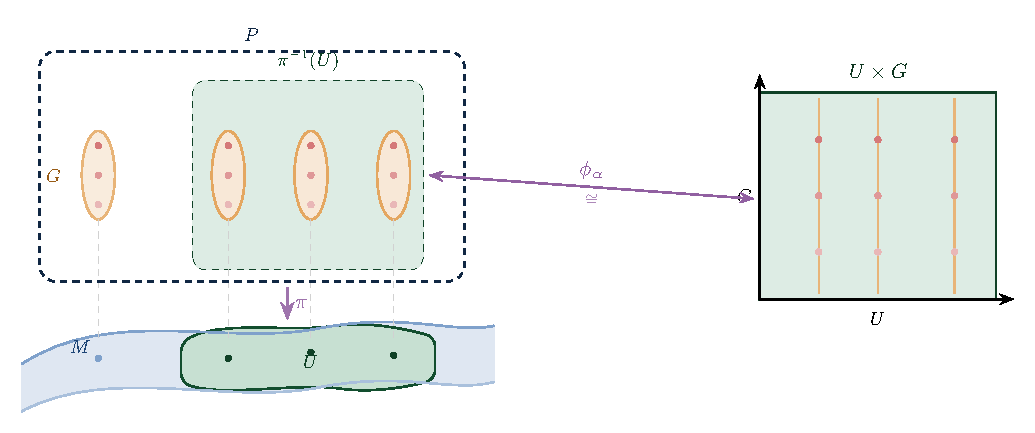
\includegraphics[width=0.7\textwidth]{images/fiber_bundle.pdf}
\caption[Structure of a principal bundle]{Structure of a principal bundle. The total space $P$ projects onto the base manifold $\mathcal{M}$ via $\pi$. Each fiber $\pi^{-1}(x)$ is diffeomorphic to the structure group $G$, and local trivializations $\phi_\alpha$ allow representing the bundle as products $U_\alpha \times G$ in open regions.}
\label{fig:fiber_bundle}
\end{figure}

\begin{example}[Bundle of Orthonormal Frames]\label{ex:fibrado_marcos}
Let $(\mathcal{M}, g)$ be an $n$-dimensional Riemannian manifold. The \textit{bundle of orthonormal frames} $\mathrm{FM}(\mathcal{M})$ is a principal bundle $(P, \mathcal{M}, \pi, O(n))$ where:
\begin{itemize}
    \item The total space $P$ consists of all orthonormal frames: $P = \{(p, e_1, \ldots, e_n) : p \in \mathcal{M}, \{e_i\} \text{ orthonormal basis of } T_p\mathcal{M}\}$
    \item The projection $\pi: P \to \mathcal{M}$ sends $(p, e_1, \ldots, e_n) \mapsto p$
    \item The group $O(n)$ acts on the right: $(p, e_1, \ldots, e_n) \cdot A = (p, \sum_j A_{j1}e_j, \ldots, \sum_j A_{jn}e_j)$
\end{itemize}
Each fiber $\pi^{-1}(p)$ is diffeomorphic to $O(n)$ and represents all possible choices of orthonormal frame at the point $p$.
\end{example}

\begin{example}[Trivial Bundle]\label{ex:fibrado_trivial}
The simplest case is the \textit{trivial bundle} $P = \mathcal{M} \times G$ with projection $\pi(p, g) = p$ and action $(p, h) \cdot g = (p, hg)$. This bundle admits a global section $s: \mathcal{M} \to P$ given by $s(p) = (p, e)$, where $e$ is the identity of $G$. Not all principal bundles admit global sections; the existence of such sections is related to the topology of the base space.
\end{example}

In the context of \gls{GDL}, the base space $\mathcal{M}$ represents the domain where the data live (for example, the sphere $S^2$ for spherical data), while the group $G$ encodes the relevant local symmetries (for example, $SO(2)$ for rotations in the tangent plane). The fiber over each point contains all the possible ``local orientations'' or ``reference frames'' at that point.

\subsection{Connections on Principal Bundles}\label{subsec:conexiones_fibrados}

A connection on a principal bundle provides a way to ``transport'' information between different fibers consistently with the structure of the group. Mathematically, a connection specifies a decomposition of the tangent space to the bundle into ``horizontal'' and ``vertical'' components.

\begin{definition}[Vertical Space]\label{def:espacio_vertical}
Let $(P, \mathcal{M}, \pi, G)$ be a principal bundle. For each $u \in P$, the \textit{vertical space} $V_u P$ is the subspace of $T_u P$ tangent to the fiber:
\[
V_u P = \ker(d\pi_u) = \{X \in T_u P : d\pi_u(X) = 0\}
\]
\end{definition}

\begin{definition}[Fundamental Vector Field]\label{def:campo_vectorial_fundamental}
Let $(P, \mathcal{M}, \pi, G)$ be a principal bundle. For each $A \in \mathfrak{g}$ (\autoref{def:algebra_lie}) and each $u \in P$, the \textit{fundamental vector field} generated by $A$ at $u$ is:
\[
A^*_u = \frac{d}{dt}\bigg|_{t=0} u \cdot \exp(tA)
\]
where $\exp: \mathfrak{g} \to G$ is the exponential map (\autoref{def:mapa_exponencial}). The curve $t \mapsto u \cdot \exp(tA)$ remains entirely within the fiber $\pi^{-1}(\pi(u))$, since the action of $G$ preserves fibers (condition (b) of \autoref{def:fibrado_principal_formal}), whence $A^*_u \in V_u P$.
\end{definition}

\begin{proposition}[Canonical Isomorphism $V_u P \cong \mathfrak{g}$]\label{prop:vertical_lie_isomorfismo}
For each $u \in P$, the map $\sigma_u: \mathfrak{g} \to V_u P$ defined by $\sigma_u(A) = A^*_u$ is an isomorphism of vector spaces.
\end{proposition}

\begin{proof}
Consider the \textit{orbit map} $\Phi_u: G \to P$ defined by $\Phi_u(g) = u \cdot g$. Its differential at the identity is $\sigma_u = (d\Phi_u)_e: T_eG = \mathfrak{g} \to T_uP$, whose image is contained in $V_uP$ by \autoref{def:campo_vectorial_fundamental}.

\textbf{Linearity.} As the differential of a smooth map, $\sigma_u = (d\Phi_u)_e$ is a linear map.

\textbf{Injectivity.} Since the action of $G$ is free, $\Phi_u$ is injective. Moreover, $\Phi_u$ is an immersion (\autoref{def:inmersion_suave}): if $(d\Phi_u)_e(A) = 0$, the curve $t \mapsto u \cdot \exp(tA)$ would have zero velocity at $t = 0$, which by freedom of the action implies $A = 0$. Hence $\sigma_u$ is injective.

\textbf{Surjectivity.} Since $\pi$ is a submersion (\autoref{def:submersion_suave}), $d\pi_u$ is surjective and $\dim V_u P = \dim \ker(d\pi_u) = \dim P - \dim \mathcal{M} = \dim G = \dim \mathfrak{g}$. An injective linear map between spaces of equal finite dimension is an isomorphism.
\end{proof}

\begin{definition}[Connection on a Principal Bundle]\label{def:conexion_fibrado}
A \textit{connection} on the principal bundle $(P, \mathcal{M}, \pi, G)$ is a 1-form (\autoref{def:1_forma_diferencial}) $\omega \in \Omega^1(P, \mathfrak{g})$ with values in the Lie algebra $\mathfrak{g}$ of $G$ that satisfies:
\begin{enumerate}
    \item \textbf{Normalization}: $\omega(A^*_u) = A$ for all $A \in \mathfrak{g}$ and $u \in P$, where $A^*$ is the fundamental vector field generated by $A$
    \item \textbf{Equivariance}: $R_g^* \omega = \mathrm{Ad}_{g^{-1}} \omega$ for all $g \in G$, where $R_g: P \to P$ denotes the right action and $\mathrm{Ad}$ is the adjoint representation
\end{enumerate}
Equivalently, a connection determines a \textit{horizontal distribution} $H_u P = \ker(\omega_u) \subset T_u P$ complementary to the vertical space, such that $T_u P = H_u P \oplus V_u P$ and $H_{u \cdot g} P = (R_g)_* H_u P$.

For a detailed exposition, see~\citep{Taubes2011}.
\end{definition}

\textbf{Geometric Interpretation.} The horizontal distribution $H_u P$ specifies which directions in the total space are ``purely spatial'' (parallel to the base) versus ``purely gauge'' (along the fiber). A curve $\tilde{\gamma}$ in $P$ is \textit{horizontal} if $\dot{\tilde{\gamma}}(t) \in H_{\tilde{\gamma}(t)} P$ for all $t$; such curves represent transport ``without rotation'' of the reference frame.

\subsection{Parallel Transport}\label{subsec:transporte_paralelo_gdl}

Parallel transport is the mechanism that allows comparing objects (vectors, tensors, or more generally elements of the bundle) located at different points of the base manifold. This comparison is essential to define operations such as convolution on non-Euclidean manifolds.

\begin{definition}[Parallel Transport on Principal Bundles]\label{def:transporte_paralelo_formal}
Let $(P, \mathcal{M}, \pi, G)$ be a principal bundle with connection $\omega$. For a smooth path $\gamma: [0,1] \to \mathcal{M}$, the \textit{parallel transport} along $\gamma$ is the map
\[
\Gamma_\gamma: \pi^{-1}(\gamma(0)) \to \pi^{-1}(\gamma(1))
\]
defined as follows: given $u_0 \in \pi^{-1}(\gamma(0))$, there exists a unique \textit{horizontal lift} $\tilde{\gamma}: [0,1] \to P$ such that:
\begin{enumerate}
    \item $\pi \circ \tilde{\gamma} = \gamma$ (the lift projects onto $\gamma$)
    \item $\tilde{\gamma}(0) = u_0$ (initial condition)
    \item $\dot{\tilde{\gamma}}(t) \in H_{\tilde{\gamma}(t)} P$ for all $t$ (horizontality)
\end{enumerate}
Then $\Gamma_\gamma(u_0) = \tilde{\gamma}(1)$.
\end{definition}

\begin{theorem}[Properties of Parallel Transport]\label{thm:propiedades_transporte}
Parallel transport satisfies the following fundamental properties:
\begin{enumerate}
    \item \textbf{Equivariance}: $\Gamma_\gamma(u \cdot g) = \Gamma_\gamma(u) \cdot g$ for all $g \in G$
    \item \textbf{Composition}: $\Gamma_{\gamma_2 * \gamma_1} = \Gamma_{\gamma_2} \circ \Gamma_{\gamma_1}$, where $\gamma_2 * \gamma_1$ denotes the concatenation of paths
    \item \textbf{Inversion}: $\Gamma_{\gamma^{-1}} = (\Gamma_\gamma)^{-1}$, where $\gamma^{-1}(t) = \gamma(1-t)$
\end{enumerate}
\end{theorem}

\begin{proof}
\textbf{Equivariance.} Let $\tilde{\gamma}$ be the horizontal lift of $\gamma$ with $\tilde{\gamma}(0) = u$, and define $\tilde{\gamma}_g(t) = \tilde{\gamma}(t) \cdot g$. We verify the three conditions of \autoref{def:transporte_paralelo_formal}:
\begin{enumerate}
    \item \textbf{Projection}: since the action of $G$ preserves fibers, $\pi(\tilde{\gamma}_g(t)) = \pi(\tilde{\gamma}(t)) = \gamma(t)$.
    \item \textbf{Initial condition}: $\tilde{\gamma}_g(0) = \tilde{\gamma}(0) \cdot g = u \cdot g$.
    \item \textbf{Horizontality}: $\dot{\tilde{\gamma}}_g(t) = (R_g)_* \dot{\tilde{\gamma}}(t) \in (R_g)_* H_{\tilde{\gamma}(t)} P = H_{\tilde{\gamma}(t) \cdot g} P$, where the last equality uses the $G$-invariance of the horizontal distribution (\autoref{def:conexion_fibrado}).
\end{enumerate}
By uniqueness of the horizontal lift, $\tilde{\gamma}_g$ is the lift of $\gamma$ from $u \cdot g$, hence $\Gamma_\gamma(u \cdot g) = \tilde{\gamma}_g(1) = \tilde{\gamma}(1) \cdot g = \Gamma_\gamma(u) \cdot g$.

\textbf{Composition.} Let $\tilde{\gamma}_1$ be the horizontal lift of $\gamma_1$ from $u_0$, with endpoint $u_1 = \tilde{\gamma}_1(1)$, and let $\tilde{\gamma}_2$ be the horizontal lift of $\gamma_2$ from $u_1$. The concatenated curve
\[
\tilde{\gamma}(t) = \begin{cases} \tilde{\gamma}_1(2t), & t \in [0, \tfrac{1}{2}], \\ \tilde{\gamma}_2(2t - 1), & t \in [\tfrac{1}{2}, 1], \end{cases}
\]
satisfies: it projects onto $\gamma_2 * \gamma_1$, starts from $u_0$ and is horizontal on each segment. By uniqueness, it is the horizontal lift of $\gamma_2 * \gamma_1$ from $u_0$, and its endpoint is $\tilde{\gamma}_2(1) = \Gamma_{\gamma_2}(\Gamma_{\gamma_1}(u_0))$.

\textbf{Inversion.} Let $\tilde{\gamma}$ be the horizontal lift of $\gamma$ from $u_0$ with endpoint $u_1 = \tilde{\gamma}(1)$. Define $\tilde{\gamma}^{-}(t) = \tilde{\gamma}(1-t)$. Then: $\pi(\tilde{\gamma}^{-}(t)) = \gamma(1-t) = \gamma^{-1}(t)$; $\tilde{\gamma}^{-}(0) = u_1$; and $\dot{\tilde{\gamma}}^{-}(t) = -\dot{\tilde{\gamma}}(1-t) \in H_{\tilde{\gamma}(1-t)}P$, since the horizontal subspaces are vector spaces. By uniqueness, $\tilde{\gamma}^{-}$ is the lift of $\gamma^{-1}$ from $u_1$, hence $\Gamma_{\gamma^{-1}}(u_1) = \tilde{\gamma}^{-}(1) = u_0 = \Gamma_\gamma^{-1}(u_1)$.

For an alternative exposition, see~\citep[Ch.~II, Prop.~3.2]{Kobayashi1996}.
\end{proof}

\begin{figure}[htbp]
\centering
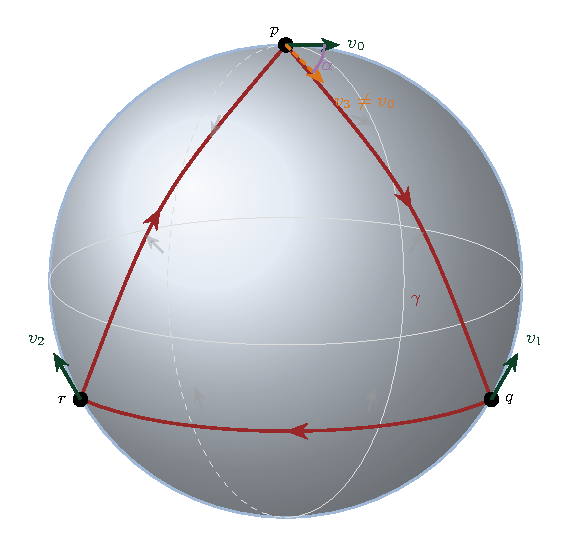
\includegraphics[width=0.85\textwidth]{images/parallel_transport.pdf}
\caption[Parallel transport and holonomy]{Parallel transport along a curve $\gamma$ on a manifold. A tangent vector at $\gamma(0)$ is transported along the path keeping itself ``parallel'' according to the connection. Holonomy arises when the vector returns to its initial point after traversing a closed loop.}
\label{fig:parallel_transport}
\end{figure}

\textbf{Differential Equation of Transport.} In terms of the connection form, the horizontal lift $\tilde{\gamma}$ satisfies the differential equation:
\[
\omega(\dot{\tilde{\gamma}}(t)) = 0
\]
If we express $\tilde{\gamma}(t) = \tilde{\gamma}_0(t) \cdot g(t)$ where $\tilde{\gamma}_0$ is a local section and $g: [0,1] \to G$, then $g(t)$ satisfies:
\[
\frac{dg}{dt} + \omega(\dot{\gamma}(t)) g(t) = 0
\]
with formal solution $g(1) = \mathcal{P} \exp\left(-\int_0^1 \omega(\dot{\gamma}(t)) dt\right) g(0)$, where $\mathcal{P}$ denotes path ordering.

\subsection{Curvature and the Structure Equation}\label{subsec:curvatura_estructura}

The curvature of a connection measures the obstruction to the integrability of the horizontal distribution, or equivalently, how much the parallel transport depends on the path chosen between two points.

\begin{definition}[Curvature of a Connection]\label{def:curvatura_formal}
Let $\omega$ be a connection on the principal bundle $(P, \mathcal{M}, \pi, G)$. The \textit{curvature} $\Omega_\omega$ is the 2-form with values in $\mathfrak{g}$ defined via the exterior derivative (\autoref{def:derivada_exterior}) and the exterior product (\autoref{def:producto_exterior_k_formas}) by:
\begin{equation}\label{eq:curvatura_definicion}
\Omega_\omega = d\omega + \frac{1}{2}[\omega \wedge \omega]
\end{equation}
where $[\omega \wedge \omega](X, Y) = [\omega(X), \omega(Y)]$ uses the Lie bracket in $\mathfrak{g}$.

More explicitly, for vector fields $X, Y$ on $P$:
\[
\Omega_\omega(X, Y) = d\omega(X, Y) + [\omega(X), \omega(Y)]
\]
The curvature is a horizontal and equivariant 2-form~\citep{Chern2000}.
\end{definition}

\begin{theorem}[Cartan's Structure Equation]\label{thm:cartan_estructura}
The curvature $\Omega_\omega$ and the connection $\omega$ satisfy \textit{Cartan's structure equation}:
\begin{equation}\label{eq:estructura_cartan}
d\omega = \Omega_\omega - \frac{1}{2}[\omega \wedge \omega]
\end{equation}
Moreover, the curvature satisfies the \textit{Bianchi identity}:
\begin{equation}\label{eq:bianchi}
d\Omega_\omega = [\omega \wedge \Omega_\omega]
\end{equation}
\end{theorem}

\begin{proof}
The structure equation is simply a rearrangement of the definition of curvature. For the Bianchi identity, we apply $d$ to both sides of \eqref{eq:curvatura_definicion}:
\[
d\Omega_\omega = d(d\omega) + \frac{1}{2}d[\omega \wedge \omega] = \frac{1}{2}([d\omega \wedge \omega] - [\omega \wedge d\omega])
\]
Substituting $d\omega = \Omega_\omega - \frac{1}{2}[\omega \wedge \omega]$ and using the properties of the Lie bracket (Jacobi identity), we obtain $d\Omega_\omega = [\omega \wedge \Omega_\omega]$.
\end{proof}

\begin{definition}[Holonomy]\label{def:holonomia}
Let $\gamma: [0,1] \to \mathcal{M}$ be a closed loop based at $p$ (that is, $\gamma(0) = \gamma(1) = p$). The \textit{holonomy} of the connection $\omega$ along $\gamma$ is the element $g_\gamma \in G$ such that:
\[
\Gamma_\gamma(u) = u \cdot g_\gamma
\]
for any $u \in \pi^{-1}(p)$.

The \textit{holonomy group} $\mathrm{Hol}_p(\omega)$ is the subgroup of $G$ generated by the holonomies of all loops based at $p$.
\end{definition}

\textbf{Curvature as Infinitesimal Holonomy.} The curvature can be interpreted as the ``infinitesimal holonomy'': for an infinitesimal loop enclosing an area $dA$ in the base manifold, the holonomy is approximately $\exp(\Omega_\omega \cdot dA)$. If the curvature vanishes ($\Omega_\omega = 0$), the connection is \textit{flat} and parallel transport is independent of the path (for homotopic paths).

\subsection{Gauge Invariance in Neural Networks}\label{subsec:invarianza_gauge_redes}

The preceding concepts have direct implications for the design of equivariant neural architectures. Modern geometric architectures must respect gauge invariances to ensure that predictions do not depend on arbitrary choices of coordinates or reference frames.

\begin{definition}[Gauge Transformation]\label{def:transformacion_gauge}
A \textit{gauge transformation} is a smooth map $g: \mathcal{M} \to G$ that assigns to each point $p \in \mathcal{M}$ an element $g(p)$ of the structure group. The set of all gauge transformations forms the \textit{gauge group}:
\[
\mathcal{G} = C^\infty(\mathcal{M}, G)
\]
with the operation of pointwise multiplication: $(g_1 \cdot g_2)(p) = g_1(p) \cdot g_2(p)$.
\end{definition}

\begin{definition}[Gauge Equivariant Function]\label{def:funcion_gauge_equivariante_gdl}
Let $\rho: G \to GL(V)$ be a representation of $G$ on a vector space $V$. A function $f: P \to V$ on the principal bundle is \textit{gauge equivariant} (or of type $\rho$) if:
\begin{equation}
f(u \cdot g) = \rho(g^{-1}) f(u)
\end{equation}
for all $u \in P$ and $g \in G$.
\end{definition}

\begin{figure}[htbp]
\centering
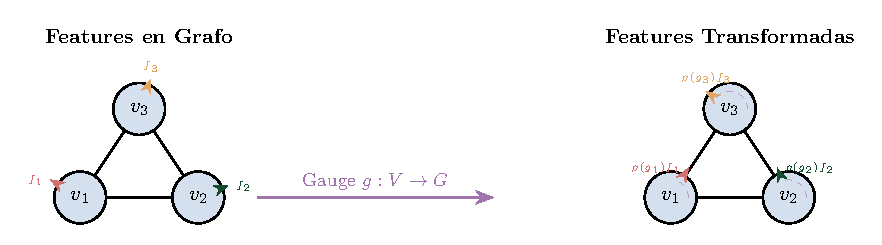
\includegraphics[width=0.75\textwidth]{images/gauge_transformation.pdf}
\caption[Gauge transformation on a graph]{Gauge transformation on a graph. A gauge transformation $g: V \to G$ independently rotates the reference frame at each vertex, transforming the features $f_i$ into $\rho(g_i)f_i$. The dashed arcs indicate the local rotation applied at each node.}
\label{fig:gauge_transformation}
\end{figure}

Gauge transformations act on the functions of the bundle, and a neural architecture $\Phi$ is gauge equivariant if it commutes with this action. Formally, if the output is a scalar (global prediction), the network is \textit{gauge invariant}:
\begin{equation}\label{eq:gauge_invariance_network}
\Phi(g \cdot f) = \Phi(f) \quad \text{for all } g: V \to G
\end{equation}
This guarantees that:

\begin{itemize}
    \item \textbf{Networks on graphs}: The output is invariant under reordering of nodes (permutation gauge)
    \item \textbf{Networks on manifolds}: Predictions are independent of the chosen parametrization or local chart
    \item \textbf{Equivariant networks}: Features transform coherently under changes of local reference frame
\end{itemize}

\textbf{Connection with Theoretical Physics.} Gauge theory in \gls{GDL} is analogous to gauge theories in physics, where the fundamental forces (electromagnetism, weak force, strong force) are described via connections on principal bundles with groups $U(1)$, $SU(2)$ and $SU(3)$ respectively. In \gls{GDL}, the gauge group encodes the local symmetries relevant to the learning problem.

The practical implementation of these ideas in concrete neural architectures, including Gauge Equivariant CNNs, is developed in detail in \autoref{sec:gauge_cnns} of \autoref{ch:cnn}.

\subsection{Examples of Gauge Equivariance in GDL}\label{subsec:ejemplos_gauge_gdl}

To illustrate the practical relevance of the concepts of gauge equivariance, we present concrete examples of how these ideas manifest in \gls{GDL} applications.

\begin{example}[Gauge Equivariance on 3D Triangulated Meshes]\label{ex:gauge_mallas_3d}
Consider a 3D surface represented as a triangular mesh $\mathcal{M} = (V, F)$, where $V$ is the set of vertices and $F$ the set of triangular faces. At each vertex $v \in V$, the tangent plane $T_v\mathcal{M}$ is well defined geometrically, but \textbf{there is no canonical choice of orthonormal basis} $(e_1^v, e_2^v)$ for this plane.

The gauge problem arises when we try to define vector fields or directional features on the mesh:
\begin{itemize}
    \item \textbf{Gauge choice}: For each vertex $v$, we choose an orthonormal basis $(e_1^v, e_2^v)$ of the tangent plane. This choice is arbitrary: any rotation $R_\theta \in SO(2)$ produces another equally valid basis.

    \item \textbf{Gauge transformation}: If we rotate the basis at vertex $v$ by an angle $\theta_v$, the components of a vector $\mathbf{u} = u_1 e_1^v + u_2 e_2^v$ transform as:
    \begin{equation}
    \begin{pmatrix} u_1' \\ u_2' \end{pmatrix} = \begin{pmatrix} \cos\theta_v & \sin\theta_v \\ -\sin\theta_v & \cos\theta_v \end{pmatrix} \begin{pmatrix} u_1 \\ u_2 \end{pmatrix}
    \end{equation}

    \item \textbf{Gauge equivariance requirement}: A neural network that processes vector features on the mesh must produce predictions that are \textbf{independent} of the choice of local bases. Mathematically, if $f: \mathcal{F}(\mathcal{M}) \to \mathcal{Y}$ is the learned function, it must satisfy:
    \begin{equation}
    f(\rho(g) \cdot \mathbf{x}) = \rho'(g) \cdot f(\mathbf{x})
    \end{equation}
    where $g = \{R_{\theta_v}\}_{v \in V}$ represents a gauge transformation (independent rotation at each vertex).
\end{itemize}
\end{example}

\begin{example}[Impact of the Gauge Choice on Predictions]\label{ex:impacto_gauge_predicciones}
To illustrate why gauge equivariance is crucial, consider a naive neural network that processes vector features on meshes without respecting gauge invariances.

\textbf{Problem:} Given a surface with a principal curvature field, we want to predict the direction of maximum curvature at each point.

\textbf{Non-gauge-equivariant architecture:} An \gls{MLP} that takes the components $(u_1, u_2)$ of vectors in local coordinates and predicts the components of the curvature direction.

\textbf{Observed failure:} If we change the orientation of the local frame at a vertex (a gauge transformation), the predictions change inconsistently:
\begin{itemize}
    \item Original frame: The network predicts direction $(\hat{d}_1, \hat{d}_2) = (0.8, 0.6)$
    \item After rotating the frame by $45^\circ$: The network predicts $(\hat{d}_1', \hat{d}_2') = (0.3, 0.9)$: a completely different direction!
\end{itemize}

\textbf{Gauge-equivariant architecture:} Networks such as Gauge Equivariant Mesh CNNs~\citep{cohen2019gaugeequivariantconvolutional} use convolutions that transform coherently under gauge changes. Their predictions satisfy:
\begin{equation}
\hat{\mathbf{d}}' = R_\theta \hat{\mathbf{d}}
\end{equation}
where $R_\theta$ is the same rotation applied to the local frame. Thus, although the \textit{numerical components} change, the predicted \textit{geometric direction} remains invariant.
\end{example}

\begin{example}[Gauge Equivariance for 3D Molecules]\label{ex:gauge_moleculas}
In the modeling of three-dimensional molecules, gauge equivariance manifests in a particularly important way for architectures that predict tensorial properties.

Consider a molecule with $n$ atoms at positions $\{\mathbf{r}_i\}_{i=1}^n \subset \mathbb{R}^3$. We want to predict the \textbf{polarizability tensor} $\boldsymbol{\alpha} \in \mathbb{R}^{3 \times 3}$, which describes how the electronic distribution responds to external electric fields.

\textbf{Fundamental physical property:} If we rotate the molecule by $R \in SO(3)$, the polarizability tensor transforms as:
\begin{equation}
\boldsymbol{\alpha}' = R \boldsymbol{\alpha} R^T
\end{equation}
This is a rank-2 tensor transformation under the group $SO(3)$.

\textbf{Gauge equivariant architectures:} Networks such as NequIP~\citep{batzner2022nequip} and Allegro represent intermediate features via \textbf{spherical tensors}, which transform according to irreducible representations of $SO(3)$. The polarizability tensor is constructed via equivariant tensor products:
\begin{equation}
\boldsymbol{\alpha} = \sum_{\ell=0,2} W_\ell \left( \mathbf{Y}^{(\ell)} \otimes \mathbf{Y}^{(\ell)} \right)
\end{equation}
where $\mathbf{Y}^{(\ell)}$ are spherical harmonics of order $\ell$ and $W_\ell$ are learned weights. This construction automatically guarantees the correct transformation under rotations.

\textbf{Practical advantage:} Predictions are physically consistent independently of the arbitrary orientation of the molecule in space, eliminating the need for data augmentation by rotations and significantly improving the efficiency of training.
\end{example}

\textbf{Synthesis of the examples.} The three preceding examples illustrate a common principle: when the data have local symmetries (gauge freedoms), neural architectures must respect these symmetries to produce physically meaningful predictions. The theory of principal bundles provides the rigorous mathematical framework for understanding and designing such architectures.


\section{Synthesis: The Unifying Framework of GDL}\label{sec:sintesis_marco_unificador}

The five fundamental G's of \gls{GDL} (Geometry, Groups, Graphs, Geodesics and Gauges) form a deeply interconnected conceptual framework: \textbf{Geometry} determines the structure of the domain and defines which \textbf{Groups} of symmetries are natural; \textbf{Graphs} discretize continuous geometries while preserving topological and spectral properties; \textbf{Geodesics} define optimal paths that respect the geometry; and \textbf{Gauges} ensure that the representations are intrinsic. From this perspective, the differences between neural architectures reflect choices about three geometric aspects: the \textbf{structure of the domain} (Euclidean spaces, graphs, manifolds), the \textbf{symmetry group} (trivial, translations, permutations) and the \textbf{connectivity} (global, fixed neighborhoods, adaptive). Traditional \glspl{ANN}, operating in $\mathbb{R}^d$ with trivial symmetries (\autoref{ch:neural_networks}), constitute the base case: they do not exploit any geometric structure, so that all invariance must be learned from the data. \gls{GDL} solves this by incorporating the symmetries directly into the architecture via the principle of equivariance (\autoref{subsec:equivarianza_invarianza}).

\subsection{Message Passing: The Unifying Framework}\label{subsec:message_passing_unificador}

\textbf{Message Passing Neural Networks} (\glspl{MPNN}) provide the unifying mathematical framework that underlies all \gls{GDL} architectures. Their conceptual foundation lies in the graph structure introduced in \autoref{def:grafo_neuronal} of \autoref{ch:neural_networks} and \autoref{def:vecindad_grafo} of \autoref{sec:grafos_discretizacion}, where the data are organized as nodes connected by edges that encode structural relationships.

This perspective reveals that the apparent differences between \glspl{ANN}, \glspl{CNN}, \glspl{Transformer} and \glspl{GNN} are manifestations of different graph topologies and connectivity strategies over the same fundamental paradigm: the propagation of information through structured neighborhoods.

\begin{definition}[Message Passing Neural Network]\label{def:mpnn_unificador}
An \textit{\gls{MPNN}} operates on a graph $\mathcal{G} = (V, E)$ with node features $\{h_v\}_{v \in V}$ and edge features $\{e_{uv}\}_{(u,v) \in E}$. The update at layer $\ell$ consists of two phases:

\begin{enumerate}
    \item \textbf{Message Passing}:
    \begin{equation}
    m_v^{(\ell+1)} = \sum_{u \in \mathcal{N}(v)} M_\ell(h_v^{(\ell)}, h_u^{(\ell)}, e_{vu})
    \end{equation}
      \item \textbf{Node Update}:
    \begin{equation}
    h_v^{(\ell+1)} = U_\ell(h_v^{(\ell)}, m_v^{(\ell+1)})
    \end{equation}
\end{enumerate}

where $M_\ell$ is the message function, $U_\ell$ is the update function, and $\mathcal{N}(v)$ is the neighborhood of node $v$ (\autoref{def:vecindad_grafo}). This formulation naturally generalizes discrete data structures. Note that this scheme operates exclusively over nodes and edges; its generalization to higher-order $k$-simplices, \textit{simplicial message passing}, is developed in \autoref{subsubsec:tdl_mpnn_general}.
\end{definition}

\begin{figure}[htbp]
\centering
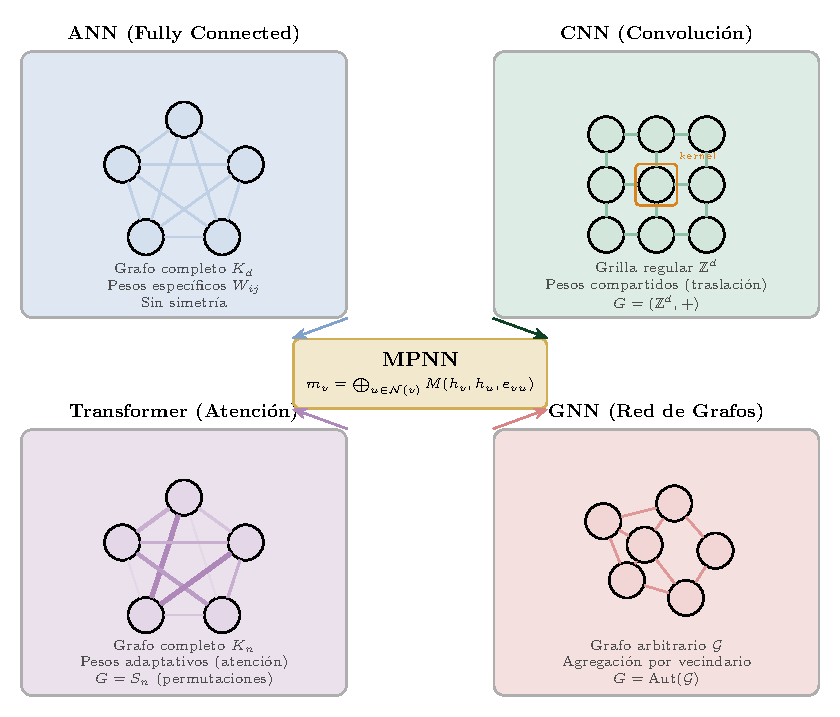
\includegraphics[width=\textwidth]{images/mpnn_unification.pdf}
\caption[Unification of architectures via Message Passing]{The four main Deep Learning architectures as instances of the \gls{MPNN} framework. \textbf{ANN}: complete graph with specific weights for each pair. \textbf{CNN}: regular grid with weights shared by translation. \textbf{Transformer}: complete graph with adaptive weights (attention). \textbf{GNN}: arbitrary graph with neighborhood aggregation. The differences reside in the graph topology and the symmetry group $G$.}
\label{fig:mpnn_unification}
\end{figure}

\subsubsection{ANNs as Trivial MPNNs}

Traditional \glspl{ANN} can be interpreted as the simplest case of \glspl{MPNN}, where each node connects to all the others with uniform weights:

\begin{proposition}[\gls{ANN} as an \gls{MPNN} on a uniform complete graph]\label{prop:ann_mpnn}
A fully connected layer $h^{(\ell+1)} = \sigma(W h^{(\ell)} + b)$ is equivalent to an \gls{MPNN} where:
\begin{itemize}
    \item \textbf{Graph}: Complete graph $K_d$ where each feature is a node
    \item \textbf{Message}: $M(h_v, h_u, e_{vu}) = W_{vu} h_u$ (specific weight for each pair)
    \item \textbf{Aggregation}: Sum over all input features
    \item \textbf{Update}: $U(h_v, m_v) = \sigma(m_v + b_v)$
\end{itemize}
\end{proposition}

\begin{proof}
Let $h^{(\ell)} \in \mathbb{R}^d$ be the feature vector at layer $\ell$. The fully connected layer computes:
\[
h_v^{(\ell+1)} = \sigma\!\left(\sum_{u=1}^{d} W_{vu} h_u^{(\ell)} + b_v\right)
\]
Interpreting each component as a node of the complete graph $K_d$, this expression coincides exactly with the message passing (\autoref{def:mpnn_unificador}) with message $M(h_v, h_u, e_{vu}) = W_{vu} h_u^{(\ell)}$, aggregation $m_v = \sum_{u \in \mathcal{N}(v)} M(\cdot) = \sum_{u=1}^d W_{vu} h_u^{(\ell)}$, and update $U(h_v, m_v) = \sigma(m_v + b_v)$.
\end{proof}

This perspective reveals why \glspl{ANN} lack \textbf{geometric inductive bias}: they treat all connections between features as equally important, ignoring any spatial, topological, or similarity structure that may exist in the data.

\subsubsection{Convolutions as Regular Message Passing}

\glspl{CNN} constitute the first nontrivial case of message passing, where the grid structure imposes a fundamental geometric inductive bias: translational equivariance.

\begin{proposition}[\gls{CNN} as an \gls{MPNN} on a regular grid]\label{prop:cnn_mpnn}
A convolutional layer over a regular grid $\mathbb{Z}^d$ with kernel of support $\mathcal{K}$ is equivalent to an \gls{MPNN} where:
\begin{itemize}
    \item \textbf{Graph}: Regular grid $\mathbb{Z}^d$ with edges $\mathcal{N}(v) = \{u \in \mathbb{Z}^d : v - u \in \mathcal{K}\}$
    \item \textbf{Message}: $M(h_v, h_u, e_{vu}) = W_{v-u} h_u$ (weights shared by relative position)
    \item \textbf{Aggregation}: Sum over the local neighborhood $m_v = \sum_{u \in \mathcal{N}(v)} W_{v-u} h_u$
    \item \textbf{Update}: $U(h_v, m_v) = \sigma(m_v + b)$
\end{itemize}
\end{proposition}

\begin{proof}
Let $h^{(\ell)}: \mathbb{Z}^d \to \mathbb{R}^{c_{\mathrm{in}}}$ be the signal at layer $\ell$ and $\{W_\delta\}_{\delta \in \mathcal{K}}$ the convolutional kernel with $W_\delta \in \mathbb{R}^{c_{\mathrm{out}} \times c_{\mathrm{in}}}$. The discrete convolution (\autoref{def:convolucion_discreta}) computes:
\[
h_v^{(\ell+1)} = \sigma\!\left(\sum_{\delta \in \mathcal{K}} W_\delta\, h_{v-\delta}^{(\ell)} + b\right) = \sigma\!\left(\sum_{u \in \mathcal{N}(v)} W_{v-u}\, h_u^{(\ell)} + b\right)
\]
where the change of variable $u = v - \delta$ transforms the sum over kernel displacements into a sum over neighbors of the grid graph. This expression coincides with the message passing (\autoref{def:mpnn_unificador}) with message $M(h_v, h_u, e_{vu}) = W_{v-u} h_u^{(\ell)}$, aggregation $m_v = \sum_{u \in \mathcal{N}(v)} M(\cdot)$ and update $U(h_v, m_v) = \sigma(m_v + b)$. The complete constructive equivalence, including the layer-by-layer correspondence by induction, is established in \autoref{thm:equivalencia_constructiva_cnn_gnn}.
\end{proof}

The key difference with respect to \glspl{ANN} is that the weights $W_{v-u}$ depend exclusively on the relative position, not on the absolute pair $(v, u)$. This weight sharing is precisely the implementation of translational equivariance as a geometric inductive bias (\autoref{theorem:convolution_translation_equivariance}), drastically reducing the number of parameters from $O(n^2 c^2)$ to $O(|\mathcal{K}| c^2)$.

\subsubsection{Attention as Adaptive Message Passing}

\glspl{Transformer} represent the complementary case: the communication weights are computed dynamically from the content of the nodes, not from their position.

\begin{proposition}[\gls{Transformer} as an \gls{MPNN} on an adaptive complete graph]\label{prop:attention_mpnn}
A self-attention layer (\autoref{def:self_attention_basica}) over a sequence of $n$ tokens is equivalent to an \gls{MPNN} where:
\begin{itemize}
    \item \textbf{Graph}: Complete graph $K_n$ where each token is a node
    \item \textbf{Message}: $M(h_i, h_j) = \alpha_{ij}\, V h_j$, with attention coefficients
    \[
    \alpha_{ij} = \frac{\exp\!\left(\frac{(Qh_i)^T(Kh_j)}{\sqrt{d_k}}\right)}{\sum_{m=1}^n \exp\!\left(\frac{(Qh_i)^T(Kh_m)}{\sqrt{d_k}}\right)}
    \]
    \item \textbf{Aggregation}: Weighted sum $m_i = \sum_{j=1}^n M(h_i, h_j)$
    \item \textbf{Update}: $U(h_i, m_i) = m_i$
\end{itemize}
\end{proposition}

\begin{proof}
Let $\{h_1, \ldots, h_n\} \subset \mathbb{R}^d$ be the input sequence and $Q, K, V \in \mathbb{R}^{d \times d_k}$ the projection matrices. The self-attention layer (\autoref{def:self_attention_basica}) computes:
\[
h_i^{(\ell+1)} = \sum_{j=1}^n \alpha_{ij}\, V h_j^{(\ell)}
= \sum_{j=1}^n \underbrace{\alpha_{ij}\, V h_j^{(\ell)}}_{M(h_i, h_j)}
\]
Identifying the complete graph $K_n$ with $\mathcal{N}(i) = \{1, \ldots, n\}$, this expression is exactly the message passing (\autoref{def:mpnn_unificador}) with message $M(h_i, h_j) = \alpha_{ij} V h_j$ and identity update $U(h_i, m_i) = m_i$. The softmax normalization guarantees $\alpha_{ij} \in (0,1)$ with $\sum_{j=1}^n \alpha_{ij} = 1$, so that the aggregation is a convex combination, unlike the uniform sum of \glspl{ANN} (\autoref{prop:ann_mpnn}) and \glspl{CNN} (\autoref{prop:cnn_mpnn}).
\end{proof}

The fundamental difference with respect to the previous architectures is that the weights $\alpha_{ij}$ are functions of the content $(h_i, h_j)$, neither fixed (\glspl{ANN}) nor dependent on the relative position (\glspl{CNN}). This adaptability enables global connectivity at the cost of quadratic complexity $O(n^2)$ in the sequence length. \autoref{ch:attention} develops the geometric extensions of this mechanism.

\subsubsection{TDL as Higher-Order Message Passing}\label{subsubsec:tdl_mpnn_general}

The three previous architectures (\glspl{ANN}, \glspl{CNN} and \glspl{Transformer}) operate exclusively over \textbf{nodes} ($0$-simplices) of a graph, propagating information along edges. \gls{TDL} breaks this restriction: it assigns signals to $k$-simplices of arbitrary order and propagates information simultaneously through the lower and upper adjacencies defined by the boundary operators. This extension incorporates a \textbf{topological inductive bias} that captures higher-order relationships inaccessible to standard message passing.

\begin{definition}[Simplicial signal]\label{def:senal_simplicial_gdl}
	A \textit{simplicial signal of order $k$} on a simplicial complex $\mathcal{K}$ is a function $\mathbf{x}: \mathcal{K}_k \to \mathbb{R}^d$ that assigns a feature vector $\mathbf{x}_\sigma \in \mathbb{R}^d$ to each $k$-simplex $\sigma \in \mathcal{K}_k$.
\end{definition}

\begin{definition}[Simplicial message passing]\label{def:mensaje_simplicial_gdl}
	\textit{Simplicial message passing} generalizes message passing on graphs (\autoref{def:mpnn_unificador}) via three types of communication for each $k$-simplex $\sigma$:
	\begin{enumerate}
		\item \textbf{Lower message} (via $\partial_k^T$): Information from $(k{-}1)$-simplices in the boundary of $\sigma$:
		\[
			\mathbf{m}_\sigma^{\mathrm{down}} = \bigoplus_{\tau \in \mathcal{B}^{\mathrm{down}}(\sigma)} M^{\mathrm{down}}\!\left(\mathbf{h}_\sigma, \mathbf{h}_\tau\right)
		\]
		where $\mathcal{B}^{\mathrm{down}}(\sigma) = \{\tau : [\partial_k^T \partial_k]_{\sigma,\tau} \neq 0\}$ are the $k$-simplices adjacent through shared faces.

		\item \textbf{Upper message} (via $\partial_{k+1}$): Information from $(k{+}1)$-simplices containing $\sigma$:
		\[
			\mathbf{m}_\sigma^{\mathrm{up}} = \bigoplus_{\rho \in \mathcal{B}^{\mathrm{up}}(\sigma)} M^{\mathrm{up}}\!\left(\mathbf{h}_\sigma, \mathbf{h}_\rho\right)
		\]
		where $\mathcal{B}^{\mathrm{up}}(\sigma) = \{\rho : [\partial_{k+1} \partial_{k+1}^T]_{\sigma,\rho} \neq 0\}$ are the $k$-simplices that share a $(k{+}1)$-simplex.

		\item \textbf{Update}:
		\[
			\mathbf{h}_\sigma' = U\!\left(\mathbf{h}_\sigma, \mathbf{m}_\sigma^{\mathrm{down}}, \mathbf{m}_\sigma^{\mathrm{up}}\right)
		\]
	\end{enumerate}
	where $\bigoplus$ denotes an aggregation function (sum, mean, maximum), $M^{\mathrm{down}}, M^{\mathrm{up}}$ are learnable message functions, and $U$ is the update function \citep{bodnar2021weisfeiler}.
\end{definition}

\begin{proposition}[\gls{TDL} as a generalized instance of the \gls{MPNN} framework]\label{prop:tdl_mpnn}
Simplicial message passing (\autoref{def:mensaje_simplicial_gdl}) is a generalized instance of the \gls{MPNN} framework (\autoref{def:mpnn_unificador}) where:
\begin{itemize}
    \item \textbf{Domain}: Simplicial complex $\mathcal{K}$, with the $k$-simplices $\sigma \in \mathcal{K}_k$ as ``nodes''
    \item \textbf{Neighborhood}: Double neighborhood $\mathcal{N}(\sigma) = \mathcal{B}^{\mathrm{down}}(\sigma) \cup \mathcal{B}^{\mathrm{up}}(\sigma)$, determined by the lower Laplacian $L_k^{\mathrm{down}} = \partial_k^T \partial_k$ and upper Laplacian $L_k^{\mathrm{up}} = \partial_{k+1} \partial_{k+1}^T$
    \item \textbf{Message}: Combination of lower and upper messages:
    \[
    M(\mathbf{h}_\sigma) = \left(\bigoplus_{\tau \in \mathcal{B}^{\mathrm{down}}(\sigma)} M^{\mathrm{down}}(\mathbf{h}_\sigma, \mathbf{h}_\tau),\; \bigoplus_{\rho \in \mathcal{B}^{\mathrm{up}}(\sigma)} M^{\mathrm{up}}(\mathbf{h}_\sigma, \mathbf{h}_\rho)\right)
    \]
    \item \textbf{Update}: $U(\mathbf{h}_\sigma, \mathbf{m}_\sigma^{\mathrm{down}}, \mathbf{m}_\sigma^{\mathrm{up}})$ learnable
\end{itemize}
In particular, for $k=0$ the standard \gls{MPNN} on graphs is recovered.
\end{proposition}

\begin{proof}
We verify the correspondence with the three components of the \gls{MPNN} framework. Let $\mathcal{K}$ be a simplicial complex and fix $k \geq 0$. We consider the graph $\mathcal{G}_k = (\mathcal{K}_k, E_k)$ whose nodes are the $k$-simplices and whose edges encode the adjacency given by $L_k$:

\textbf{(1) Message.} For each $k$-simplex $\sigma$, simplicial message passing (\autoref{def:mensaje_simplicial_gdl}) computes two messages:
\[
\mathbf{m}_\sigma^{\mathrm{down}} = \bigoplus_{\tau \in \mathcal{B}^{\mathrm{down}}(\sigma)} M^{\mathrm{down}}(\mathbf{h}_\sigma, \mathbf{h}_\tau), \qquad
\mathbf{m}_\sigma^{\mathrm{up}} = \bigoplus_{\rho \in \mathcal{B}^{\mathrm{up}}(\sigma)} M^{\mathrm{up}}(\mathbf{h}_\sigma, \mathbf{h}_\rho)
\]
Defining $\mathcal{N}(\sigma) = \mathcal{B}^{\mathrm{down}}(\sigma) \cup \mathcal{B}^{\mathrm{up}}(\sigma)$ and the joint message $\widetilde{M}(\mathbf{h}_\sigma, \mathbf{h}_\nu) = M^{\mathrm{down}}(\mathbf{h}_\sigma, \mathbf{h}_\nu)$ if $\nu \in \mathcal{B}^{\mathrm{down}}(\sigma)$ and $\widetilde{M}(\mathbf{h}_\sigma, \mathbf{h}_\nu) = M^{\mathrm{up}}(\mathbf{h}_\sigma, \mathbf{h}_\nu)$ if $\nu \in \mathcal{B}^{\mathrm{up}}(\sigma)$, this takes the form $m_\sigma = \bigoplus_{\nu \in \mathcal{N}(\sigma)} \widetilde{M}(\mathbf{h}_\sigma, \mathbf{h}_\nu)$, which corresponds to the message phase of \autoref{def:mpnn_unificador}.

\textbf{(2) Aggregation.} The operator $\bigoplus$ (sum, mean or maximum) plays the role of the permutation-invariant aggregation function of the \gls{MPNN} scheme.

\textbf{(3) Update.} The function $U(\mathbf{h}_\sigma, \mathbf{m}_\sigma^{\mathrm{down}}, \mathbf{m}_\sigma^{\mathrm{up}})$ corresponds directly to the update function $U_\ell$ of the \gls{MPNN} framework.

\textbf{Reduction to $k=0$.} For $0$-simplices (nodes), $\partial_0 = 0$ implies $L_0^{\mathrm{down}} = 0$, so $\mathcal{B}^{\mathrm{down}}(v) = \emptyset$ and the lower message vanishes. The upper message reduces to $\mathbf{m}_v^{\mathrm{up}} = \bigoplus_{u \in \mathcal{B}^{\mathrm{up}}(v)} M^{\mathrm{up}}(\mathbf{h}_v, \mathbf{h}_u)$, where $\mathcal{B}^{\mathrm{up}}(v) = \{u : [\partial_1 \partial_1^T]_{vu} \neq 0\} = \mathcal{N}(v)$ is the standard neighborhood of node $v$ in the graph $1$-skeleton. This recovers exactly the classical message passing on graphs.
\end{proof}

\begin{proposition}[Expressiveness of simplicial message passing]\label{prop:expresividad_simplicial}
	Simplicial message passing is strictly more expressive than message passing on graphs. There exist pairs of non-isomorphic simplicial complexes whose 1-skeletons are identical (and therefore indistinguishable by \glspl{MPNN}), but which simplicial networks distinguish correctly thanks to the higher-order topological information.
\end{proposition}

This result, proved by \citet{bodnar2021weisfeiler}, shows that the topological information encoded in the boundary operators $\partial_k$ provides a discriminative power that surpasses the limitations of the \gls{WL} test established in \autoref{subsubsec:test_weisfeiler_leman}.

This proposition closes the arc of unification of the \gls{MPNN} framework: while \glspl{ANN}, \glspl{CNN} and \glspl{Transformer} encode spatial or relational inductive \textit{biases} over nodes, \gls{TDL} introduces a \textbf{higher-order topological inductive bias} that allows capturing interactions between triangles, tetrahedra and arbitrary $k$-simplices. As shown in \autoref{prop:expresividad_simplicial}, this topological bias provides expressive power strictly superior to that of message passing on graphs, surpassing the \gls{WL} barrier \citep{bodnar2021weisfeiler, hajij2023topological}.

\subsection{Expressive Power and Synthesis of the Unifying Framework}\label{subsec:poder_expresivo_sintesis}

The expressive power of message-passing-based architectures is fundamentally limited by deep theoretical considerations:

\subsubsection{The Weisfeiler-Leman Test}\label{subsubsec:test_weisfeiler_leman}

The \textbf{Weisfeiler-Leman test} (\gls{WL}) is a classical algorithm originally proposed in 1968~\citep{weisfeiler1968reduction} to determine whether two graphs are isomorphic via an iterative process of \textbf{refined coloring}. Its importance in \gls{GDL} lies in the fact that it establishes a fundamental theoretical upper bound for the expressive power of \glspl{MPNN}.

\begin{definition}[Weisfeiler-Leman algorithm (1-WL)]\label{def:weisfeiler_leman}
Let $G = (V, E)$ be a graph with $n$ vertices. The \textit{order-1 Weisfeiler-Leman algorithm} (1-WL) consists of the following iterative coloring process:
\begin{enumerate}
    \item \textbf{Initialization} ($t=0$): Assign to each node $v \in V$ an initial color $c^{(0)}(v)$, typically identical for all nodes (or based on node labels if they exist).

    \item \textbf{Iterative refinement}: At each iteration $t \geq 0$, update the color of each node according to:
    \begin{equation}\label{eq:wl_update}
    c^{(t+1)}(v) = \mathrm{HASH}\left(c^{(t)}(v), \{\{c^{(t)}(u) : u \in \mathcal{N}(v)\}\}\right)
    \end{equation}
    where $\mathcal{N}(v)$ is the neighborhood of $v$, $\{\{\cdot\}\}$ denotes a multiset, and $\mathrm{HASH}$ is an injective function that assigns a new unique color to each distinct pair (old color, multiset of neighboring colors).

    \item \textbf{Convergence}: The algorithm terminates when the color partition stabilizes, that is, when $c^{(t+1)}(v) = c^{(t)}(v)$ for all $v \in V$. This occurs in at most $n$ iterations.

    \item \textbf{Final histogram}: The result of the algorithm is the \textit{color histogram} $\mathbf{h}(G) = (|\{v : c^{(T)}(v) = k\}|)_{k}$, which counts how many nodes have each final color.
\end{enumerate}
\end{definition}

\begin{definition}[WL-equivalence]\label{def:wl_equivalencia}
Two graphs $G_1$ and $G_2$ are \textit{WL-equivalent}, denoted $G_1 \equiv_{\mathrm{WL}} G_2$, if the 1-WL algorithm produces the same color histogram for both graphs.
\end{definition}

\begin{figure}[htbp]
\centering
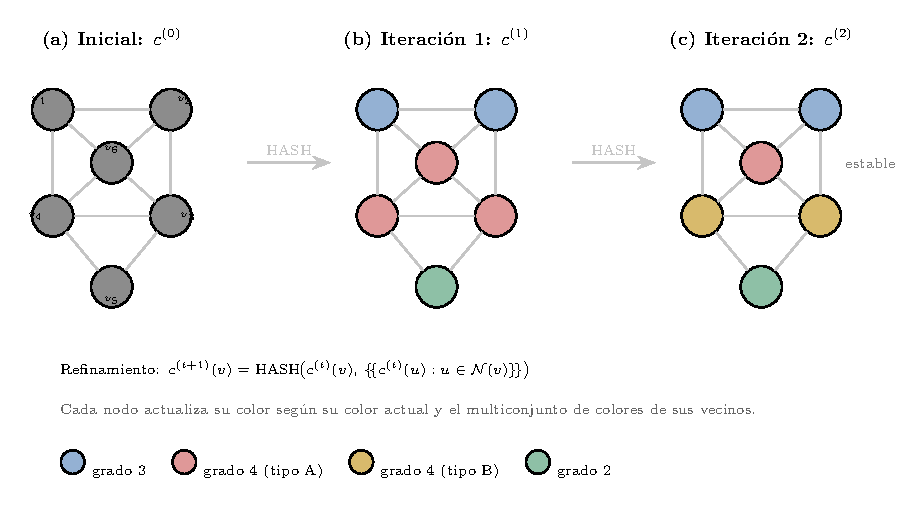
\includegraphics[width=\textwidth]{images/weisfeiler_leman.pdf}
\caption[Weisfeiler-Leman color refinement]{Example of the 1-WL color refinement test on a graph of 6 nodes. (a) Uniform initial coloring. (b) After the first iteration, the nodes are distinguished by degree: blue (degree~3), red (degree~4), green (degree~2). (c) The second iteration refines according to the multiset of neighboring colors: $v_3$ and $v_4$ (yellow) are separated from $v_6$ (red) because their neighborhoods have distinct color compositions.}
\label{fig:weisfeiler_leman}
\end{figure}

The deep connection between the WL test and graph networks was rigorously established by~\citet{xu2019how} and~\citet{morris2019weisfeiler}:

\begin{theorem}[WL-MPNN equivalence]\label{thm:wl_mpnn_equivalencia}
Let $\mathcal{G}$ be a class of graphs and let $\mathcal{A}$ be an \gls{MPNN} with injective aggregation and update functions. Then:
\begin{enumerate}
    \item \textbf{Upper bound}: $\mathcal{A}$ cannot distinguish graphs that are WL-equivalent. That is, if $G_1 \equiv_{\mathrm{WL}} G_2$, then $\mathcal{A}(G_1) = \mathcal{A}(G_2)$.

    \item \textbf{Optimality}: There exists an \gls{MPNN} (specifically, a Graph Isomorphism Network or GIN) that is \textit{as expressive as} the WL test. That is, if $G_1 \not\equiv_{\mathrm{WL}} G_2$, there exists a configuration of weights such that $\mathcal{A}(G_1) \neq \mathcal{A}(G_2)$.
\end{enumerate}
\end{theorem}

\begin{proof}[Proof sketch]
The key idea is the structural correspondence between one iteration of the WL algorithm and one layer of an \gls{MPNN}:

\textbf{WL $\rightarrow$ MPNN}: The WL refinement $c^{(t+1)}(v) = \mathrm{HASH}(c^{(t)}(v), \{\{c^{(t)}(u)\}\})$ maps directly to a message-aggregation-update layer:
\[
h_v^{(t+1)} = \phi\left(h_v^{(t)}, \bigoplus_{u \in \mathcal{N}(v)} \psi(h_u^{(t)})\right)
\]
If $\phi$ and $\oplus$ are sufficiently expressive (for example, sum over unique embeddings followed by an MLP), they exactly reproduce the behavior of $\mathrm{HASH}$.

\textbf{MPNN $\rightarrow$ WL}: Conversely, if two graphs are WL-equivalent, they have the same sequence of color partitions. Since \glspl{MPNN} can only aggregate neighborhood information, they cannot ``break'' the symmetry that the WL test preserves.

The complete proof requires showing that the sum aggregator over sufficiently unique embeddings is injective, which is established via the Universal Approximation Theorem for sets~\citep{zaheer2017deepsets}.
\end{proof}

\begin{example}[Non-isomorphic graphs indistinguishable by WL]\label{ex:grafos_wl_indistinguibles}
The simplest example of non-isomorphic graphs that the 1-WL test cannot distinguish are regular graphs of the same degree and size:

Consider two hexagonal graphs:
\begin{itemize}
    \item $G_1$: A cycle of 6 nodes (hexagon): $C_6$
    \item $G_2$: Two disjoint triangles: $K_3 \sqcup K_3$
\end{itemize}

Both graphs have 6 nodes, 6 edges, and all nodes have degree 2. The WL algorithm assigns:
\begin{enumerate}
    \item Iteration 0: All nodes receive the same initial color $c^{(0)} = 1$.
    \item Iteration 1: Each node sees neighbors with color 1, multiset $\{\{1, 1\}\}$. New color: $c^{(1)} = \mathrm{HASH}(1, \{\{1,1\}\}) = 2$ for all.
    \item Convergence: The partition does not change. Final histogram: $\mathbf{h}(G_1) = \mathbf{h}(G_2) = (6)$.
\end{enumerate}

However, $G_1 \not\cong G_2$: the cycle $C_6$ is connected while $K_3 \sqcup K_3$ has two connected components. This limitation shows that standard \glspl{MPNN} cannot detect the global connectivity of regular graphs.

\textbf{Implication for GDL}: If a task requires distinguishing molecules with similar global structures but different connectivities (for example, structural isomers), standard \glspl{MPNN} may fail systematically.
\end{example}

\subsubsection{Over-smoothing: Spectral Analysis}\label{subsubsec:oversmoothing}

\autoref{thm:wl_mpnn_equivalencia} delimits which graphs \glspl{MPNN} can distinguish, but says nothing about what happens when we stack many message-passing layers. The answer, known as \textit{\gls{oversmoothing}}~\citep{li2018deeper}, is that the node representations converge to a uniform value, losing all discriminative capacity. This phenomenon admits an elegant spectral explanation that connects directly with the tools developed in \autoref{subsec:analisis_espectral_grafos_gdl}.

\begin{definition}[Dirichlet energy on graphs]\label{def:energia_dirichlet_grafos}
	Let $\mathcal{G} = (V, E)$ be a graph with Laplacian $L_G$ and let $H \in \mathbb{R}^{n \times d}$ be a matrix of node features ($n = |V|$, $d$ channels). The \textit{Dirichlet energy} of $H$ is
	\[
		E(H) = \operatorname{tr}(H^T L_G H) = \sum_{c=1}^{d} \mathbf{h}_c^T L_G \mathbf{h}_c = \sum_{c=1}^{d} \sum_{(i,j) \in E} W_{ij}(h_{ic} - h_{jc})^2,
	\]
	where $\mathbf{h}_c$ denotes the $c$-th column of $H$.
\end{definition}

The last equality follows from the quadratic form of \autoref{prop:propiedades_algebraicas_laplaciano}. The Dirichlet energy measures the total variation of the signals $H$ over the graph: $E(H) = 0$ if and only if $H$ is constant on each connected component. This is the discrete version of the Dirichlet energy mentioned in \autoref{subsec:analisis_espectral_grafos_gdl}.

\begin{proposition}[Linear MPNN as discrete diffusion]\label{prop:mpnn_difusion}
	Consider an \gls{MPNN} (\autoref{def:mpnn_unificador}) with mean aggregation and no nonlinearity:
	\[
		h_v^{(\ell+1)} = (1 - \alpha) h_v^{(\ell)} + \alpha \sum_{u \in \mathcal{N}(v)} \frac{h_u^{(\ell)}}{\deg(v)},
	\]
	with $\alpha \in (0, 1]$. Let $\tilde{L} = D^{-1}L_G = I - D^{-1}A$ be the random-walk Laplacian, which shares its spectrum with the symmetric normalized Laplacian of \autoref{def:laplaciano_normalizado}. Then the update is written in matrix form as
	\begin{equation}\label{eq:difusion_discreta}
		H^{(\ell+1)} = (I - \alpha \tilde{L})\, H^{(\ell)}.
	\end{equation}
\end{proposition}

\begin{proof}
	For each node $v$, the update rule is:
	\begin{align*}
		h_v^{(\ell+1)} &= (1-\alpha) h_v^{(\ell)} + \alpha \sum_{u \sim v} \frac{h_u^{(\ell)}}{\deg(v)} = h_v^{(\ell)} - \alpha\left(h_v^{(\ell)} - \sum_{u \sim v} \frac{h_u^{(\ell)}}{\deg(v)}\right)\\
		&= h_v^{(\ell)} - \alpha (D^{-1}L_G\, H^{(\ell)})_v = h_v^{(\ell)} - \alpha (\tilde{L}\, H^{(\ell)})_v,
	\end{align*}
	where we use that $\tilde{L} = D^{-1}L_G = I - D^{-1}A$ and that $(D^{-1}A H)_v = \sum_{u \sim v} h_u / \deg(v)$.
\end{proof}

Equation~\eqref{eq:difusion_discreta} is the temporal discretization of the heat equation $\partial_t H = -\alpha \tilde{L} H$ on the graph. Iterating $\ell$ layers, $H^{(\ell)} = (I - \alpha \tilde{L})^\ell H^{(0)}$, which progressively diffuses the signals.

\begin{theorem}[Exponential convergence of over-smoothing]\label{thm:oversmoothing_convergencia}
	Let $\mathcal{G}$ be a connected graph with eigenvalues of the normalized Laplacian $0 = \lambda_1 < \lambda_2 \leq \cdots \leq \lambda_n$ (\autoref{prop:propiedades_espectrales_laplaciano_grafos}) and $\alpha \in (0, 1/\lambda_n)$. Then the Dirichlet energy of the representations after $\ell$ layers of the linear \gls{MPNN} satisfies
	\begin{equation}\label{eq:oversmoothing_bound}
		E\bigl(H^{(\ell)}\bigr) \leq (1 - \alpha\lambda_2)^{2\ell}\, E\bigl(H^{(0)}\bigr).
	\end{equation}
	In particular, $E(H^{(\ell)}) \to 0$ exponentially as $\ell \to \infty$: all representations converge to a single vector.
\end{theorem}

\begin{proof}
	Let $\{u_k\}_{k=1}^n$ be the orthonormal basis of eigenvectors of $L_{\mathrm{sym}} = D^{-1/2} L_G D^{-1/2}$ with eigenvalues $\lambda_k$ (\autoref{def:transformada_fourier_grafos}). We define $\mathbf{f}_c = D^{1/2}\mathbf{h}_c$ for each column of $H$, so that $\mathbf{h}_c^T L_G \mathbf{h}_c = \mathbf{f}_c^T L_{\mathrm{sym}} \mathbf{f}_c$. The Fourier transform decomposes $\mathbf{f}_c = \sum_{k=1}^n \hat{f}_{c,k}\, u_k$.

	The diffusion operator satisfies $D^{1/2}(I - \alpha \tilde{L})D^{-1/2} = I - \alpha L_{\mathrm{sym}}$, which has eigenvalues $1 - \alpha\lambda_k$. After $\ell$ iterations, the spectral coefficients of $\mathbf{f}_c^{(\ell)} = D^{1/2}\mathbf{h}_c^{(\ell)}$ are scaled by $(1-\alpha\lambda_k)^\ell \hat{f}_{c,k}$.

	The Dirichlet energy in the spectral domain is (\autoref{thm:interpretacion_frecuencial_autovectores}):
	\[
		E(H^{(\ell)}) = \sum_{c=1}^d \mathbf{f}_c^{(\ell)T} L_{\mathrm{sym}} \mathbf{f}_c^{(\ell)} = \sum_{c=1}^d \sum_{k=2}^n \lambda_k (1-\alpha\lambda_k)^{2\ell} |\hat{f}_{c,k}|^2,
	\]
	where the term $k=1$ disappears because $\lambda_1 = 0$. Since $\alpha < 1/\lambda_n$, we have $|1-\alpha\lambda_k| < 1$ for $k \geq 2$, and in particular $|1-\alpha\lambda_k| \leq 1-\alpha\lambda_2$ for all $k \geq 2$ (the maximum is attained at $\lambda_2$, the lowest nontrivial frequency). Therefore:
	\[
		E(H^{(\ell)}) \leq (1-\alpha\lambda_2)^{2\ell} \sum_{c=1}^d \sum_{k=2}^n \lambda_k |\hat{f}_{c,k}|^2
		= (1-\alpha\lambda_2)^{2\ell}\, E(H^{(0)}).
	\]
	Since $0 < \alpha\lambda_2 < 1$, the factor $(1-\alpha\lambda_2)^{2\ell} \to 0$ exponentially.
\end{proof}

\begin{remark}[Geometric interpretation of over-smoothing]\label{rem:oversmoothing_geometrico}
	The convergence rate $(1-\alpha\lambda_2)^{2\ell}$ is controlled by the \textbf{spectral gap} $\lambda_2$, the second eigenvalue of the Laplacian. Graphs with large $\lambda_2$ (such as expanders) converge faster to the uniform state, while poorly connected graphs ($\lambda_2 \approx 0$) better preserve the diversity of representations. This is the exact discrete version of heat diffusion on Riemannian manifolds (\autoref{rem:laplace_beltrami_gdl}), where the spectral gap of the Laplace-Beltrami operator controls the mixing rate.

	Among the strategies to mitigate \gls{oversmoothing} stand out residual connections (which preserve the original signal), layer normalization, and topological approaches such as Neural Sheaf Diffusion~\citep{bodnar2022neural}, where scalar diffusion is replaced by a diffusion on sheaves that allows each edge to transport information in different vector spaces.
\end{remark}

\subsubsection{Over-squashing: Topological Bottlenecks}\label{subsubsec:oversquashing}

If \gls{oversmoothing} arises from the loss of high-frequency signal, the complementary phenomenon of \textit{\gls{oversquashing}} is the inability to propagate information over long distances. Intuitively, the information from a distant node must be compressed exponentially in order to ``pass'' through the bottlenecks of the graph.

\begin{definition}[Jacobian sensitivity of an MPNN]\label{def:sensibilidad_mpnn}
	Consider an \gls{MPNN} with representations $h_v^{(\ell)} \in \mathbb{R}^d$. The \textit{sensitivity} of node $v$ with respect to node $u$ after $\ell$ layers is
	\[
		S_{vu}^{(\ell)} = \left\|\frac{\partial h_v^{(\ell)}}{\partial h_u^{(0)}}\right\|,
	\]
	where the norm is the operator norm of the Jacobian matrix $\partial h_v^{(\ell)} / \partial h_u^{(0)} \in \mathbb{R}^{d \times d}$.
\end{definition}

If $S_{vu}^{(\ell)} \approx 0$, node $v$ is essentially insensitive to the input of node $u$: any information that $u$ carries has been lost during propagation.

\begin{proposition}[Exponential decay of sensitivity]\label{prop:oversquashing_exponencial}
	Consider an \gls{MPNN} with Lipschitz message and update functions with constants $c_M$ and $c_U$ respectively, and let $\hat{A} = D^{-1}A$ be the random-walk transition matrix on $\mathcal{G}$. Then for any nodes $v, u \in V$:
	\begin{equation}\label{eq:oversquashing_bound}
		S_{vu}^{(\ell)} \leq (c_U \cdot c_M)^\ell\, [\hat{A}^\ell]_{vu}.
	\end{equation}
	In particular, if $d_\mathcal{G}(v, u) > \ell$ (\autoref{def:distancia_geodesica_grafo}), then $[\hat{A}^\ell]_{vu} = 0$ and the sensitivity is exactly zero.
\end{proposition}

\begin{proof}[Proof sketch]
	We proceed by induction on $\ell$. For $\ell = 1$ and nodes $v \neq u$,
	since $h_v^{(1)} = U(h_v^{(0)}, m_v^{(1)})$, the full chain rule is
	\[
		\frac{\partial h_v^{(1)}}{\partial h_u^{(0)}}
		= \frac{\partial U}{\partial h_v^{(0)}}
		  \cdot \underbrace{\frac{\partial h_v^{(0)}}{\partial h_u^{(0)}}}_{=\,0 \text{ if } v \neq u}
		+ \frac{\partial U}{\partial m_v}
		  \cdot \frac{\partial m_v}{\partial h_u^{(0)}}
		= \frac{\partial U}{\partial m_v}
		  \cdot \frac{\partial m_v}{\partial h_u^{(0)}}.
	\]
	The second factor is nonzero only if $u \in \mathcal{N}(v)$, in which case
	the Lipschitz constant of $M$ contributes $c_M$ and the degree
	normalization contributes the factor $1/\deg(v) = [\hat{A}]_{vu}$. Thus
	$S_{vu}^{(1)} \leq c_U c_M [\hat{A}]_{vu}$.

	For the inductive step, we apply the multivariable chain rule:
	\[
		\frac{\partial h_v^{(\ell+1)}}{\partial h_u^{(0)}} = \sum_{w \in \mathcal{N}(v) \cup \{v\}} \frac{\partial h_v^{(\ell+1)}}{\partial h_w^{(\ell)}} \cdot \frac{\partial h_w^{(\ell)}}{\partial h_u^{(0)}}.
	\]
	Bounding each factor by the Lipschitz constants and using the inductive hypothesis for $\partial h_w^{(\ell)} / \partial h_u^{(0)}$, we obtain the matrix product $\hat{A}^{\ell+1}$ that records all paths of length $\ell+1$ from $u$ to $v$.
\end{proof}

\begin{remark}[Curvature and over-squashing]\label{rem:curvatura_oversquashing}
	The bound~\eqref{eq:oversquashing_bound} reveals that the topology of the graph, encoded in $\hat{A}^\ell$, is the determining factor of \gls{oversquashing}. \citet{topping2022understanding} formalize this connection via the \textbf{discrete Ricci curvature} (Ollivier): edges $(u,v)$ with negative Ricci curvature correspond to bottlenecks where $[\hat{A}^\ell]_{vu}$ decays rapidly. This is the discrete version of the Jacobi equation in Riemannian geometry (\autoref{rem:significado_curvatura}): negative sectional curvature causes geodesics to diverge, reducing the ``volume of information'' that can propagate. Topping et al. propose \textit{rewiring} the graph via Ricci flow, adding edges in regions of negative curvature to alleviate the bottlenecks, an example of how differential geometry prescribes solutions to problems of \glspl{GNN}.
\end{remark}

\subsubsection{The k-WL Hierarchy and Extensions}\label{subsubsec:jerarquia_kwl}

\autoref{thm:wl_mpnn_equivalencia} establishes that \glspl{MPNN} are as expressive as the 1-WL test, which operates over individual nodes. A natural extension is to consider higher-order tests that operate over tuples of nodes.

\begin{definition}[Order-$k$ Weisfeiler-Leman test]\label{def:k_wl}
	The \textit{$k$-\gls{WL} test} operates over $k$-tuples of nodes $\bar{v} = (v_1, \ldots, v_k) \in V^k$ \citep{morris2019weisfeiler}. An initial coloring $c^{(0)}(\bar{v})$ is defined based on the isomorphism type of the subtuple, along with the iterative refinement:
	\[
		c^{(t+1)}(\bar{v}) = \mathrm{HASH}\!\left(c^{(t)}(\bar{v}),\, \bigl\{\!\!\bigl\{ \bigl(c^{(t)}(\bar{v}[w/1]), \ldots, c^{(t)}(\bar{v}[w/k])\bigr) : w \in V \bigr\}\!\!\bigr\}\right),
	\]
	where $\bar{v}[w/i]$ denotes the tuple obtained by replacing the $i$-th component of $\bar{v}$ by $w$.
\end{definition}

\begin{proposition}[Strict expressiveness hierarchy]\label{prop:jerarquia_kwl}
	The Weisfeiler-Leman tests form a strictly increasing hierarchy in expressive power:
	\[
		1\text{-WL} \subsetneq 2\text{-WL} \subsetneq 3\text{-WL} \subsetneq \cdots
	\]
	That is, for each $k \geq 1$ there exist graphs that $k$-WL does not distinguish but $(k+1)$-WL does. The computational complexity of the $k$-WL test is $O(n^k \log n)$ per iteration, where $n = |V|$.
\end{proposition}

\begin{proof}
	The proof of the strict separation requires techniques from finite model logic (in particular, the connection with the Immerman-Lander logic $C^k$) and exceeds the scope of this thesis; see~\citet{morris2019weisfeiler} for the details. The complexity $O(n^k \log n)$ follows directly from the iterative refinement: there are $n^k$ tuples, each iteration requires inspecting $n$ substitutions per tuple, and stabilization occurs in at most $O(n^k)$ iterations with cost $O(\log n)$ for the hash.
\end{proof}

There are various strategies to overcome the 1-WL barrier without incurring the exponential cost of $k$-WL:
\begin{itemize}
	\item \textbf{Simplicial message passing}: As shown by \autoref{prop:expresividad_simplicial}, operating over simplicial complexes ($k$-chains) allows surpassing 1-WL by incorporating higher-order topological information.
	\item \textbf{Structural encodings}: Adding positional encodings based on eigenvectors of the Laplacian (\autoref{def:transformada_fourier_grafos}) or random walks breaks the symmetry of the nodes.
	\item \textbf{Spectral Graph Transformers}: Architectures such as~\citet{kreuzer2021spectral} combine global attention with spectral encodings, connecting the ideas of \autoref{subsec:analisis_espectral_grafos_gdl} with the attention mechanisms of \autoref{ch:attention}.
\end{itemize}

\medskip

The three limitations analyzed (\gls{oversmoothing}, \gls{oversquashing} and the WL barrier) are manifestations of the fundamentally \textbf{local} character of message passing: each layer only propagates information one hop. \gls{oversmoothing} shows that too many layers destroy the discriminative signal; \gls{oversquashing} shows that too few layers prevent long-range communication; and the WL barrier shows that certain global patterns are undetectable locally. The geometric tools developed in this chapter (spectral analysis, discrete curvature, higher-order topology) not only \textit{diagnose} these limitations but also \textit{prescribe} concrete solutions.

From this perspective, we can synthesize the unifying framework that emerges from the preceding analysis. The unifying perspective of \gls{GDL} reveals a natural progression in the geometric sophistication of neural architectures: \glspl{ANN} operate in Euclidean spaces with trivial symmetries; \glspl{CNN} introduce \textbf{spatial inductive bias} via locality and translational equivariance; \glspl{Transformer} generalize this via \textbf{global adaptive connectivity}, where attention implements message passing with dynamic weights; and this paradigm extends naturally to arbitrary graphs with complex topologies.

This theoretical framework is predictive, not merely descriptive: it suggests design principles for new hybrid architectures based on the geometric foundations established. Chapters~\ref{ch:cnn} and~\ref{ch:attention} delve into these architectures from their specific geometric perspectives, providing the complete mathematical foundations for equivariant convolutions and geometric attention mechanisms. Geometry is not optional in Deep Learning: it is the fundamental organizing principle that determines which architectures are effective for which types of data and problems.
